\chapter{Higher Dimensional Eigenvalues}

In this chapter we verify the correctness and examine the performance of the Rayleigh Quotient Fixed Point methods for higher-dimensional problems. We consider realistic two- and three-dimensional problems involving fuel rods and fuel assemblies. For higher dimensions, the phase space of the neutron transport equation is a function of two $(x, y)$ or three $(x, y, z)$ spatial variables and two $\hat{\Omega} = (\mu, \eta)$ or three $\hat{\Omega} =  (\mu, \eta, \xi)$ angular variables defined as the $x$-, $y$-, and $z$-direction cosines. For higher-dimensional Cartesian geometry, the two-dimensional and three-dimensional alpha-eigenvalue neutron transport equations are given by Eq.~\ref{eq:2DAlpha} and Eq.~\ref{eq:3DAlpha}, respectively:

\begin{multline}
\bigg [ \mu \frac{\partial}{\partial x} + \eta \frac{\partial}{\partial y} + \frac{\alpha}{v(E)} + \sigma(x,y,E) \bigg ] \psi(x,y,\hat{\Omega},E) \\ = \frac{\chi(E)}{2} \int_{0}^{\infty} \diff E' \nu(E') \sigma_{f}(x,y,E') \int_{2\pi} \diff \hat{\Omega}' \, \psi(x,y, \hat{\Omega}', E) \\ + \frac{1}{2\pi} \int_{0}^{\infty} \diff E' \sigma_{s}(x, y, E' \rightarrow E) \int_{2\pi} \diff \hat{\Omega}' \, \psi(x,y, \hat{\Omega}',E),
\label{eq:2DAlpha}
\end{multline}

\begin{multline}
\bigg [ \mu \frac{\partial}{\partial x} + \eta \frac{\partial}{\partial y} + \xi \frac{\partial}{\partial z} + \frac{\alpha}{v(E)} + \sigma(x,y,z,E) \bigg ] \psi(x,y,z,\hat{\Omega}, E) \\ = \frac{\chi(E)}{2} \int_{0}^{\infty} \diff E' \nu(E') \sigma_{f}(x,y,z,E') \int_{4\pi} \diff \hat{\Omega}' \, \psi(x,y,z, \hat{\Omega}',E) \\ + \frac{1}{4\pi} \int_{0}^{\infty} \diff E' \sigma_{s}(x, y, z, E' \rightarrow E) \int_{4\pi} \diff \hat{\Omega}' \, \psi(x,y,z, \hat{\Omega}',E).
\label{eq:3DAlpha}
\end{multline}
The three-dimensional $k$-effective eigenvalue neutron transport equation is given by \ref{eq:3Dk}:

\begin{multline}
\bigg [ \mu \frac{\partial}{\partial x} + \eta \frac{\partial}{\partial y} + \xi \frac{\partial}{\partial z} + \sigma(x,y,z,E) \bigg ] \psi(x,y,z,\hat{\Omega}, E) \\ = \frac{1}{k}\frac{\chi(E)}{2} \int_{0}^{\infty} \diff E' \nu(E') \sigma_{f}(x,y,z,E') \int_{4\pi} \diff \hat{\Omega}' \, \psi(x,y,z, \hat{\Omega}',E) \\ + \frac{1}{4\pi} \int_{0}^{\infty} \diff E' \sigma_{s}(x, y, z, E' \rightarrow E) \int_{4\pi} \diff \hat{\Omega}' \, \psi(x,y,z, \hat{\Omega}',E).
\label{eq:3Dk}
\end{multline}

We also consider two-dimensional cylindrical geometry problems. For cylindrical geometry problems, the complexity is increased due to the fact that for one spatial dimension, two angular variables are required to describe the angular flux. For two-dimensional cylindrical problems, the alpha-eigenvalue neutron transport equation is given by 

\begin{multline}
\frac{\mu}{\rho} \frac{\partial}{\partial \rho} (\rho \psi) + \xi \frac{\partial \psi}{\partial z} - \frac{1}{\rho} \frac{\partial}{\partial \omega} (\eta \psi) + \frac{\alpha}{v(E)} \psi(\rho,\hat{\Omega},E) + \sigma(\rho,E) \psi(\rho,\hat{\Omega}E) \\ = \frac{\chi(E)}{2} \int_{0}^{\infty} \diff E' \nu(E') \sigma_{f}(\rho,E') \int_{4\pi} \diff \hat{\Omega}' \, \psi(\rho, \hat{\Omega}',E) \\ + \frac{1}{4\pi} \int_{0}^{\infty} \diff E' \sigma_{s}(\rho, E' \rightarrow E) \int_{4\pi} \diff \hat{\Omega}' \, \psi(\rho, \hat{\Omega}',E),
\label{eq:2DCylAlpha}
\end{multline}
where $\rho$ is the radial distance from the origin and $\mu = (1-\xi^{2})^{1/2} \cos \omega$ and $\eta = (1-\xi^{2})^{1/2}\sin \omega$ (Figure \ref{fig:Cyl2D}).

\begin{figure}[!htbp]
\centering
\resizebox{0.55\textwidth}{!}{
	%usepackage{tikz}   %TikZ is required for this to work.  Make sure this exists before the next line

%\usepackage{3dplot} %requires 3dplot.sty to be in same directory, or in your LaTeX installation

%\usepackage[active,tightpage]{preview}  %generates a tightly fitting border around the work
%\PreviewEnvironment{tikzpicture}
%\setlength\PreviewBorder{2mm}

%\begin{document}

%Angle Definitions
%-----------------

%set the plot display orientation
%synatax: \tdplotsetdisplay{\theta_d}{\phi_d}
\tdplotsetmaincoords{60}{110}

%define polar coordinates for some vector
%TODO: look into using 3d spherical coordinate system
\pgfmathsetmacro{\rvec}{1.2}
\pgfmathsetmacro{\thetavec}{45}
\pgfmathsetmacro{\phivec}{60}

%start tikz picture, and use the tdplot_main_coords style to implement the display 
%coordinate transformation provided by 3dplot
\begin{tikzpicture}[scale=5,tdplot_main_coords]

%set up some coordinates 
%-----------------------
\coordinate (O) at (0,0,0);

%determine a coordinate (P) using (r,\theta,\phi) coordinates.  This command
%also determines (Pxy), (Pxz), and (Pyz): the xy-, xz-, and yz-projections
%of the point (P).
%syntax: \tdplotsetcoord{Coordinate name without parentheses}{r}{\theta}{\phi}
\tdplotsetcoord{P}{\rvec}{\thetavec}{\phivec}

%draw figure contents
%--------------------

%draw the main coordinate system axes
\draw[thick,->] (0,0,0) -- (1,0,0) node[anchor=north east]{$x$};
\draw[thick,->] (0,0,0) -- (0,1,0) node[anchor=north west]{$y$};
\draw[thick,->] (0,0,0) -- (0,0,1) node[anchor=south]{$z$};

%draw a vector from origin to point (P) 
\draw[thick,->,color=black] (O) -- (P);

%draw projection on xy plane, and a connecting line
%\draw[ color=black] (O) -- (Pxy) node[anchor=north]{$r$};
\draw[ color=black] (O) -- (Pxy);
\node at (0.5,0.5,0) {$\rho$};
\node at (0.0,0.53,0.2) {$z$};
\node at (0.0,0.25,0.35) {$\vec{r}$};
\draw[ color=black] (P) -- (Pxy);

\node at (0,1,0.65) {$\omega$};
\node at (0,0.75,0.53) {$\mu$};
\node at (0,0.5,0.7) {$\xi$};
\node at (0,0.8,0.82) {$\eta$};

%draw the angle \phi, and label it
%syntax: \tdplotdrawarc[coordinate frame, draw options]{center point}{r}{angle}{label options}{label}
\tdplotdrawarc{(O)}{0.2}{0}{\phivec}{anchor=north}{$\theta$}


%set the rotated coordinate system so the x'-y' plane lies within the
%"theta plane" of the main coordinate system
%syntax: \tdplotsetthetaplanecoords{\phi}
\tdplotsetthetaplanecoords{\phivec}

%draw theta arc and label, using rotated coordinate system
%\tdplotdrawarc[tdplot_rotated_coords]{(0,0,0)}{0.5}{0}{\thetavec}{anchor=south west}{$\theta$}

%draw some dashed arcs, demonstrating direct arc drawing
%\draw[dashed,tdplot_rotated_coords] (\rvec,0,0) arc (0:90:\rvec);
%\draw[dashed] (\rvec,0,0) arc (0:90:\rvec);

%set the rotated coordinate definition within display using a translation
%coordinate and Euler angles in the "z(\alpha)y(\beta)z(\gamma)" euler rotation convention
%syntax: \tdplotsetrotatedcoords{\alpha}{\beta}{\gamma}
%\tdplotsetrotatedcoords{\phivec}{\thetavec}{0}
\tdplotsetrotatedcoords{0}{0}{0}

%translate the rotated coordinate system
%syntax: \tdplotsetrotatedcoordsorigin{point}
\tdplotsetrotatedcoordsorigin{(P)}

%use the tdplot_rotated_coords style to work in the rotated, translated coordinate frame
\draw[color=red,thick,tdplot_rotated_coords,->] (0,0,0) -- (-.6,0,0) node[anchor=south]{$-\hat{e}_{\theta}$};
\draw[color=red,thick,tdplot_rotated_coords,->] (0,0,0) -- (0,.5,0) node[anchor=west]{$\hat{e}_{\rho}$};
\draw[color=red,thick,tdplot_rotated_coords,->] (0,0,0) -- (0,0,.5) node[anchor=south]{$\hat{e}_{z}$};

%WARNING:  coordinates defined by the \coordinate command (eg. (O), (P), etc.)
%cannot be used in rotated coordinate frames.  Use only literal coordinates.  

%draw some vector, and its projection, in the rotated coordinate frame
\draw[thick,->,color=blue,tdplot_rotated_coords] (0,0,0) -- (-.3,.3,.1) node[anchor=south]{$\hat{\Omega}$};
\draw[dashed,color=blue,tdplot_rotated_coords] (-.3,.3,.1) -- (-.3,.3,0);
\draw[dashed,color=blue,tdplot_rotated_coords] (-.3,.3,0) -- (0,.3,0);
\draw[dashed,color=blue,tdplot_rotated_coords] (-.3,.3,0) -- (-.3,0,0);
\draw[dashed,color=blue,tdplot_rotated_coords] (-.3,.3,0) -- (0,0,0);

\draw[dashed,color=blue,tdplot_rotated_coords] (-.3,.3,.1) -- (-.3,-.11,.1);
%\draw[dashed,color=blue,tdplot_rotated_coords] (.2,.2,0) -- (.2,.2,.2);

%show its phi arc and label
%\tdplotdrawarc[tdplot_rotated_coords,color=blue]{(0,0,0)}{0.2}{0}{45}{anchor=north west,color=black}{$\phi'$}

%change the rotated coordinate frame so that it lies in its theta plane.
%Note that this overwrites the original rotated coordinate frame
%syntax: \tdplotsetrotatedthetaplanecoords{\phi'}
\tdplotsetrotatedthetaplanecoords{45}

%draw theta arc and label
%\tdplotdrawarc[tdplot_rotated_coords,color=blue]{(0,0,0)}{0.2}{0}{55}{anchor=south west,color=black}{$\theta'$}

\end{tikzpicture}
%	% 3D axis with spherical coordinates
\tdplotsetmaincoords{60}{110}
\begin{tikzpicture}[scale=3,tdplot_main_coords]
 
  % variables
  \def\rvec{1.4}
  \def\thetavec{45}
  \def\phivec{60}
 
  % axes
  \coordinate (O) at (0,0,0);
  \draw[thick,->] (0,0,0) -- (1,0,0) node[anchor=north east]{$x$};
  \draw[thick,->] (0,0,0) -- (0,1,0) node[anchor=north west]{$y$};
  \draw[thick,->] (0,0,0) -- (0,0,1) node[anchor=south]{$z$};
 
  % vectors
  \tdplotsetcoord{P}{\rvec}{\thetavec}{\phivec}
  \draw[-stealth,black] (O)  -- (P) node[above right] {$P$};
  \draw[dashed,black]   (O)  -- (Pxy);
  \draw[dashed,black]   (P)  -- (Pxy);
  %\draw[dashed,red]   (Py) -- (Pxy);
 
  % arcs
  \tdplotdrawarc[->]{(O)}{0.2}{0}{\phivec}
    {anchor=north}{$\theta$}
  \tdplotsetthetaplanecoords{\phivec}
  \tdplotdrawarc[->,tdplot_rotated_coords]{(0,0,0)}{0.5}{0}{\thetavec}
    {anchor=south west}{$\theta$}
    
    \tdplotsetthetaplanecoords{\phivec}
\tdplotsetcoord{P}{\rvec}{\thetavec}{\phivec}
\tdplotsetrotatedcoords{0}{0}{0}

%translate the rotated coordinate system
%syntax: \tdplotsetrotatedcoordsorigin{point}
\tdplotsetrotatedcoordsorigin{(P)}
\draw[thick,tdplot_rotated_coords,->] (0,0,0) -- (-.5,0,0) node[anchor=north west]{$x'$};
\draw[thick,tdplot_rotated_coords,->] (0,0,0) -- (0,.5,0) node[anchor=west]{$y'$};
\draw[thick,tdplot_rotated_coords,->] (0,0,0) -- (0,0,.5) node[anchor=south]{$z'$};
\tdplotsetrotatedthetaplanecoords{45}
 
\end{tikzpicture}
	}
	\caption{Cylindrical Space-Angle Coordinate System in Three Dimensions}
	\label{fig:Cyl2D}
\end{figure}
%Various homogeneous and heterogeneous slab geometry problems with vacuum boundary conditions were modeled in ARDRA. These slab media problems consist of multiplying and non-multiplying materials with thicknesses $\Delta$. Alpha- and $k$-effective eigenvalues were calculated and the number of transport sweeps compared to various methods such as the critical search method and the power method. To verify the correctness of the Rayleigh quotient fixed point method (RQFP), the method was compared to various methods such as Green's Function Method (GFM) and Direct Evaluation (DE) and compared to other discrete ordinate neutron transport codes such as PARTISN/DANT.

Reactor fuel assemblies and fuel pins were modeled in ARDRA. These benchmark problems consisted of detailed heterogeneous domains with many nuclei of interest to reactor design and physics. The higher dimension geometry of the problems along with the many energy-group cross section libraries allowed for analysis of the Rayleigh Quotient Fixed Point method for alpha- and $k$-effective eigenvalue problems in situations where assumptions of positivity might no longer be valid.

\section{Critical Cylinder Benchmark Problems}

We consider homogeneous and heterogeneous two-dimensional cylindrical problems in this section. In the homogeneous case, a critical \textit{infinite cylinder} domain is modeled with critical radius $r_{c}$ and height $z_{c}$ to approximate an infinite cylinder in the $z$-direction (Figure~\ref{fig:CylCritRadius}). In the heterogeneous case, an infinite cylinder is surrounded by some reflector (such as water). The inclusion of the reflector introduces regions in the problem domain where fission is not possible and only downscattering is allowed. This violates the conditions necessary for primitivity (see Section~\ref{sec:PrimPos}). We find that the inclusion of non-fissile reflector material does not impact the ability of the Rayleigh Quotient Fixed Point method for alpha- and $k$-effective eigenvalue problems to obtain the fundamental eigenpair.

\begin{figure}[!htbp]
	\centering
	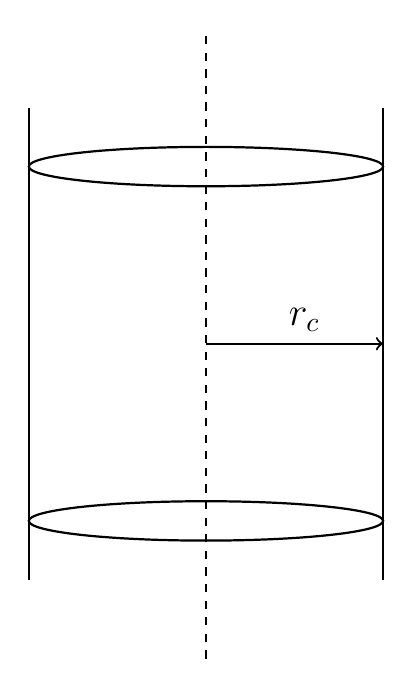
\begin{tikzpicture}[text centered]
    \begin{scope}[thick,font=\Large]

    \draw [-] (-2.25,-3) -- (-2.25,3) {};
%    \draw [-] (2.5,-3) -- (0.5,3) {};
    
    \draw [dashed] (0.0,-4) -- (0,4) {};
    \draw (2.25,-3.) -- (2.25,3) {};
    
    \draw [->] (0,0) -- (2.25,0) node [align=center] at (1.25,0.3) {$r_{c}$};
    
    \draw (0,2.25) ellipse (2.25 and 0.25);
    \draw (0,-2.25) ellipse (2.25 and 0.25);

    \end{scope}
\end{tikzpicture}
	\caption{Critical Radius of Infinite Cylinder}
	\label{fig:CylCritRadius}
\end{figure}

\subsection{Homogeneous Critical Cylinder Problems}

Five exactly critical homogeneous cylinder problems from Sood \cite{sood2003analytical} were considered with cross sections listed in Table~\ref{table:SoodCyl}. These problems consisted of plutonium, uranium-235, and heavy-water/uranium mixture cylinders with critical radii listed in Table~\ref{table:SoodCylRes}. All problem cross-sections were one-group and two problems included anisotropic scattering.

The number of transport sweeps necessary for convergence for the RQFP and critical search method can be seen in Table~\ref{table:SoodCylAlpha}. For the plutonium problem, the RQFP method required 38 sweeps to converge the alpha-eigenvalue and eigenvector. The critical search method required 461 transport sweeps. In this particular problem the RQFP method reduced the number of transport sweeps necessary by a factor of 10. For the uranium-235 problem, the RQFP method required 45 transport sweeps as compared to 455 sweeps for the critical search method, a factor of 10 reduction. For the heavy-water/uranium mixture, the number of transport sweeps required to converge the eigenpair increased dramatically. For this set of cross section data, 319 transport sweeps were required by the RQFP method to converge the fundamental mode and eigenvalue. The critical search method was not able to converge the alpha-eigenvalue as the system as modeled was slightly subcritical. For the uranium-235 cross sections with anisotropic scattering, the RQFP method was found to take 41 and 53 transport sweeps each. The critical search method was unable to converge these methods despite the fact that the systems were slightly supercritical. The critical search method was unable to converge the alpha-eigenvalue and eigenvector due to the fact that the $k$-effective eigenvalue goes negative in the interpolation part of the algorithm.

The number of transport sweeps necessary for convergence for the RQFP and power method with fission source update can be seen in Table~\ref{table:SoodCylK}. The RQFP method requires a similar number of sweeps to converge the $k$-effective eigenvalue problem except for the heavy-water/uranium mixture problem. In this case, the RQFP method requires 320 transport sweeps to only 121 transport sweeps for the power method with fission source update. This implies that the convergence rate of the RQFP method is much more strongly influenced by the amount of scattering in the system as compared to the power method. In all cases, the number of sweeps required by the RQFP method to converge the $k$-effective eigenvalue was similar to the number of sweeps required to converge the alpha-eigenvalue problem. 

\begin{table}[!htbp]
	\caption{One-Group Cross Sections for Infinite Cylinder Critical Problems (cm$^{-1}$) \cite{sood2003analytical}}
	\label{table:SoodCyl}
	\centering\ra{1.3}
    \begin{tabular}{*6c}
        \toprule
	Cross Section Set & $\sigma$ & $\nu \sigma_{f}$ & $\sigma_{s0}$ & $\sigma_{s1}$ & $v$ [cm/s] \\ 
        \midrule
	PUb & 0.32640 & 0.231744 & 0.225216 & 0.0 & 1 \\
	U-235a & 0.32640 & 0.176256 & 0.248064 & 0.0 & 1 \\
	U-D$_{2}$O & 0.54628 & 0.0928676 & 0.464338 & 0.0 & 1 \\
	U-235a Anisotropic & 0.32640 & 1.76256 & 0.248064 & 0.04432 & 1 \\
	U-235b Anisotropic & 0.32640 & 1.76256 & 0.248064 & 0.212160 & 1 \\
        \bottomrule
    \end{tabular}
\end{table}

\begin{table}[!htbp]
	\caption{Calculated Eigenvalues and Transport Sweep Comparisons for Critical Infinite Cylinder Problems in \cite{sood2003analytical}}
	\label{table:SoodCylRes}
	\begin{subtable}[h]{1.0\textwidth}
	\centering\ra{1.3}
	\begin{tabular}{@{}ccccc@{}}\toprule
	& & & \multicolumn{2}{c}{Transport Sweeps} \\
	\cmidrule{4-5} Cross Section Set & r$_{c}$ [cm] & Calculated $\alpha$ [s$^{-1}$] & RQFP & Critical Search\\
	\midrule
	PUb & 4.279960 & $3.783833 \times 10^{-4}$ & 38 & 461 \\
	U-235a & 5.284935 & $ 1.973082 \times 10^{-4}$ & 45 & 455 \\
	U-D$_{2}$O & 16.554249 & $ -1.007328 \times 10^{-4}$ &  319 & * \\
	U-235a Anisotropic & 5.514296811 & $ 2.012672 \times 10^{-4}$ & 41 & * \\
	U-235b Anisotropic & 6.940205668 & $ 1.906997 \times 10^{-4}$ & 53 & * \\ 
	\bottomrule
	\multicolumn{5}{l}{*Did Not Converge} \\
	\end{tabular}
	\caption{Alpha-Eigenvalue: Comparison of RQFP and Critical Search Transport Sweeps}
	\label{table:SoodCylAlpha}
	\end{subtable}%
	\vspace{0.25cm}
	\begin{subtable}[h]{1.0\textwidth}
	\centering\ra{1.3}
	\begin{tabular}{@{}ccccc@{}}\toprule
	& & & \multicolumn{2}{c}{Transport Sweeps} \\
	\cmidrule{4-5} Cross Section Set & r$_{c}$ [cm] & Calculated $k_{\text{eff}}$ & RQFP & Power Method \\
	\midrule
	PUb & 4.279960 & 1.001419 & 43 & 40 \\
	U-235a & 5.284935 & 1.000989 & 49 & 42 \\
	U-D$_{2}$O & 16.554249 & 0.998935 & 320 & 121 \\
	U-235a Anisotropic & 5.514296811 & 1.000997 & 48 & 40 \\
	U-235b Anisotropic & 6.940205668 & 1.000870 & 37  & 43 \\
	\bottomrule
	\multicolumn{5}{l}{$M = 500$, $L = 10$, Tolerance = $10^{-12}$} \\
	\end{tabular}
	\caption{$k$-Effective: Comparison of RQFP and Power Method Transport Sweeps}
	\label{table:SoodCylK}
	\end{subtable}
\end{table}

\clearpage

\section{Two- and Three-Dimensional Cartesian Benchmark Problems}

We consider three versions of the MOX Fuel Assembly 3D Extension Case from the \textit{Benchmark on Deterministic Transport Calculations Without Spatial Homogenisation} \cite{lewis2001benchmark}. The benchmark geometry is a three-dimensional representation of sixteen assembly (quarter core symmetry) C5 MOX fuel assembly problem described in \cite{cavarec1994oecd}. The benchmark problem is meant to provide a challenging test of the ability of three-dimensional methods to handle spatial heterogeneities. 

The benchmark problem materials consist of seven materials: UO$_{2}$ fuel-clad, 4.3\% MOX fuel, 7.0\% MOX fuel, 8.7\% MOX fuel, the fission chamber, the guide tube, and the moderator. Each material has a seven energy cross section set with energy group boundaries and group speeds listed in Table~\ref{table:SevenGrpBounds}.The seven energy group, isotropic scattering cross sections for the UO$_{2}$ fuel-clad are provided in Table~\ref{table:MOX-FuelClad}. The seven energy group, isotropic scattering cross sections for the three enrichments of MOX are listed in Table~\ref{table:MOX-43}, Table~\ref{table:MOX-7}, and Table~\ref{table:MOX-87} while the cross sections for the fission chamber, guide tube, and moderator are listed in Table~\ref{table:MOX-Fission}, Table~\ref{table:MOX-Guide}, and Table~\ref{table:MOX-Mod}, respectively.

The quarter core has dimensions 64.26 cm by 64.26 cm by 214.20 cm. Each fuel pin cell has width 1.26 cm and the radius of the fuel cylinder is 0.54cm.The quarter core model consists to two types of assembly, UO$_{2}$ and MOX surrounded by moderator as seen in Figure~\ref{fig:CoreConfig}. Each fuel assembly has a pin layout as shown in Figure~\ref{fig:FuelPinAssembly}. Reflected boundary conditions are imposed on the bottom and right quarter core boundaries. Vacuum boundary conditions are imposed on the top and left edges of the quarter core. The $k$-effective eigenvalue of the system benchmark problem is $k = 1.186550$.

Three variations of the benchmark problem were considered. Two two-dimensional variants of the benchmark problem were modeled where reflective boundary conditions were placed on the top and bottom of the quarter core. In the first problem, a coarse spatial homogenization was done on a high-fidelity geometric model created for the LLNL Monte Carlo code COG \cite{buck1993cog} and the problem solved using ARDRA. In the second case, a finer spatial homogenization was done the high-fidelity geometric model. Finally, a full three-dimensional calculation with coarse spatial homogenization was done. The performance of the RQFP method for alpha- and $k$-effective eigenvalues was investigated for all problems and compared to traditional eigenvalue solution methods in the field.

\begin{figure}[!htbp]
\centering
\resizebox{0.55\textwidth}{!}{
	\input{Figures/HigherDimEigen/CoreConfig.tex}
	}
	\caption{Assembly Layout for MOX Fuel Assembly Benchmark}
	\label{fig:CoreConfig}
\end{figure}

\begin{figure}[!htbp]
\centering
  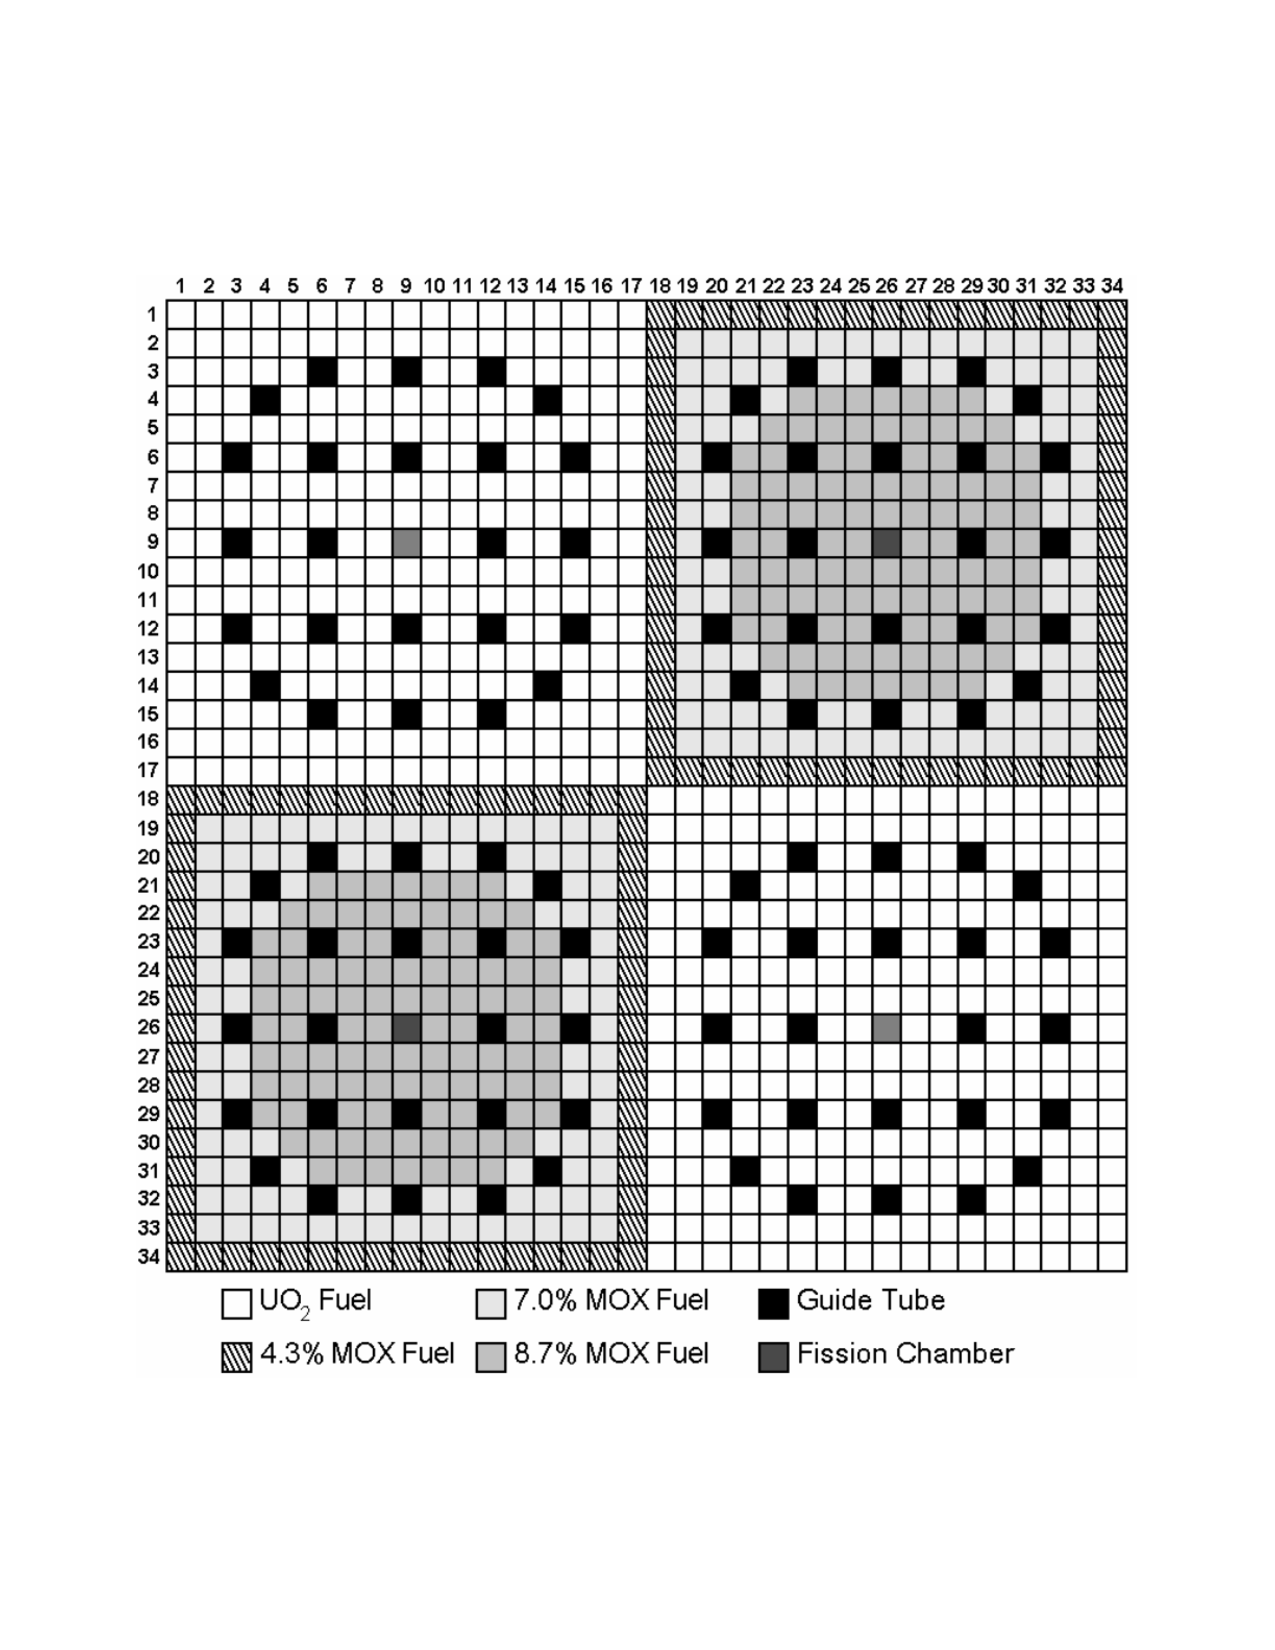
\includegraphics[trim=2cm 4cm 2cm 4cm,clip=true,width=.55\linewidth]{Figures/HigherDimEigen/FuelPinAssembly}
\caption{Fuel Pin Layout for MOX Fuel Assembly Benchmark From \cite{lewis2001benchmark}}
  \label{fig:FuelPinAssembly}
\end{figure}

\begin{sidewaysfigure}
\begin{table}[H]
    \centering
    \caption{C5G7MOX Energy Group Boundaries (MeV) and Speeds (cm/s)}
    \label{table:SevenGrpBounds}
    \resizebox{1.0\textwidth}{!}{
    \begin{tabular}{*5c}
        \toprule
	Energy Group $g$ & Upper Energy Boundary & Midpoint Energy & Lower Energy Boundary & Speed \\
        \midrule
 0 & 2.000000E+01 & 1.750000E+01 & 1.500000E+01 & 5.692375E+03 \\
 1 & 1.500000E+01 & 1.250000E+01 & 1.000000E+01 & 4.817827E+03 \\
 2 & 1.000000E+01 & 7.500000E+00 & 5.000000E+00 & 3.711626E+03 \\
 3 & 5.000000E+00 & 2.550000E+00 & 1.000000E-01 & 1.762394E+03 \\
 4 & 1.000000E-01 & 5.050000E-02 & 1.000000E-03 & 2.405592e+02 \\
 5 & 1.000000E-03 & 5.050000E-04 & 1.000000E-05 & 2.405663E+01 \\
 6 & 1.000000E-05 & 5.000500e-06 & 1.000000E-09 & 2.208836E+00 \\
        \bottomrule
        & & & &
    \end{tabular}}
 \end{table}
 \end{sidewaysfigure}

\begin{sidewaysfigure}
\begin{table}[H]
    \caption{C5G7MOX Cross Sections - UO$_{2}$ Fuel-Clad}
    \label{table:MOX-FuelClad}
	\begin{subtable}[h]{1.0\textwidth}
    \centering
    \resizebox{1.0\textwidth}{!}{
    \begin{tabular}{*8c}
        \toprule
	Energy Group $g$ & $\sigma_{g}$ & $\sigma_{g,tr}$ & $\sigma_{a,g}$ & $\sigma_{\gamma,g}$ & $\sigma_{f,g}$ & $\nu_{g}$ & $\chi_{g}$ \\ 
        \midrule
0 & 2.12450E-01 & 1.77949E-01 & 8.02480E-03 & 8.12740E-04 & 7.21206E-03 & 2.78145E+00 & 5.87910E-01 \\
1 & 3.55470E-01 & 3.29805E-01 & 3.71740E-03 & 2.89810E-03 & 8.19301E-04 & 2.47443E+00 & 4.11760E-01 \\
2 & 4.85540E-01 & 4.80388E-01 & 2.67690E-02 & 2.03158E-02 & 6.45320E-03 & 2.43383E+00 & 3.39060E-04 \\
3 & 5.59400E-01 & 5.54367E-01 & 9.62360E-02 & 7.76712E-02 & 1.85648E-02 & 2.43380E+00 & 1.17610E-07 \\
4 & 3.18030E-01 & 3.11801E-01 & 3.00200E-02 & 1.22116E-02 & 1.78084E-02 & 2.43380E+00 & 0.00000E+00 \\
5 & 4.01460E-01 & 3.95168E-01 & 1.11260E-01 & 2.82252E-02 & 8.30348E-02 & 2.43380E+00 & 0.00000E+00 \\
6 & 5.70610E-01 & 5.64406E-01 & 2.82780E-01 & 6.67760E-02 & 2.16004E-01 & 2.43380E+00 & 0.00000E+00 \\
        \bottomrule
        & & & & & & & 
    \end{tabular}}
        \caption{UO$_{2}$ Fuel-Clad Cross Sections --  (cm$^{-1}$)}
 \end{subtable} %
\begin{subtable}[h]{1.0\textwidth}
%\begin{table}[H]
    \centering
    \resizebox{1.0\textwidth}{!}{
    \begin{tabular}{*8c}
        \toprule
	$g'$, $g$ & 1 & 2 & 3 & 4 & 5 & 6 & 7 \\
        \midrule
1 & 1.27537E-01 & 4.23780E-02 & 9.43740E-06 & 5.51630E-09 & 0.00000E+00 & 0.00000E+00 & 0.00000E+00 \\
2 & 0.00000E+00 & 3.24456E-01 & 1.63140E-03 & 3.14270E-09 & 0.00000E+00 & 0.00000E+00 & 0.00000E+00 \\
3 & 0.00000E+00 & 0.00000E+00 & 4.50940E-01 & 2.67920E-03 & 0.00000E+00 & 0.00000E+00 & 0.00000E+00 \\
4 & 0.00000E+00 & 0.00000E+00 & 0.00000E+00 & 4.52565E-01 & 5.56640E-03 & 0.00000E+00 & 0.00000E+00 \\
5 & 0.00000E+00 & 0.00000E+00 & 0.00000E+00 & 1.25250E-04 & 2.71401E-01 & 1.02550E-02 & 1.00210E-08 \\
6 & 0.00000E+00 & 0.00000E+00 & 0.00000E+00 & 0.00000E+00 & 1.29680E-03 & 2.65802E-01 & 1.68090E-02 \\
7 & 0.00000E+00 & 0.00000E+00 & 0.00000E+00 & 0.00000E+00 & 0.00000E+00 & 8.54580E-03 & 2.73080E-01 \\
        \bottomrule
        & & & & & & & 
    \end{tabular}}
        \caption{UO$_{2}$ Fuel-Clad Scattering Block (cm$^{-1}$)}
  \end{subtable}
\end{table}
\end{sidewaysfigure}

\begin{sidewaysfigure}
\begin{table}[H]
    \caption{C5G7MOX Cross Sections - 4.3\% MOX Fuel}
        \label{table:MOX-43}
  \begin{subtable}[h]{1.0\textwidth}
%\begin{table}[H]
    \centering
    \resizebox{1.00\textwidth}{!}{
    \begin{tabular}{*8c}
        \toprule
	Energy Group $g$ & $\sigma_{g}$ & $\sigma_{g,tr}$ & $\sigma_{a,g}$ & $\sigma_{\gamma,g}$ & $\sigma_{f,g}$ & $\nu_{g}$ & $\chi_{g}$ \\ 
        \midrule
0 & 2.11920E-01	 &	1.78731E-01 &	8.43390E-03 &	8.06860E-04 &	7.62704E-03 &	2.85209E+00 &	5.87910E-01 \\
1 & 3.55810E-01	 &	3.30849E-01 &	3.75770E-03 &	2.88080E-03 &	8.76898E-04 &	2.89099E+00 &	4.11760E-01 \\
2 & 4.88900E-01	 &	4.83772E-01 &	2.79700E-02 &	2.22717E-02 &	5.69835E-03 &	2.85486E+00 &	3.39060E-04 \\
3 & 5.71940E-01	 &	5.66922E-01 &	1.04210E-01 &	8.13228E-02 &	2.28872E-02 &	2.86073E+00 &	1.17610E-07 \\
4 & 4.32390E-01	 &	4.26227E-01 &	1.39940E-01 &	1.29177E-01 &	1.07635E-02 &	2.85447E+00 &	0.00000E+00 \\
5 & 6.84950E-01	 &	6.78997E-01 &	4.09180E-01 &	1.76423E-01 &	2.32757E-01 &	2.86415E+00 &	0.00000E+00 \\
6 & 6.88910E-01	 &	6.82852E-01 &	4.09350E-01 &	1.60382E-01 &	2.48968E-01 &	2.86780E+00 &	0.00000E+00 \\
        \bottomrule
        & & & & & & & 
    \end{tabular}}
        \caption{4.3\% MOX Fuel -- Clad Cross Sections (cm$^{-1}$)}
  \end{subtable}
  \begin{subtable}[h]{1.0\textwidth}
%\begin{table}[H]
    \centering
    \resizebox{1.00\textwidth}{!}{
    \begin{tabular}{*8c}
        \toprule
	$g'$, $g$ & 1 & 2 & 3 & 4 & 5 & 6 & 7 \\
        \midrule
0 & 1.28876E-01	 &	4.14130E-02 &	8.22900E-06 &	5.04050E-09 &	0.00000E+00 &	0.00000E+00 &	0.00000E+00 \\
1 & 0.00000E+00	 &	3.25452E-01 &	1.63950E-03 &	1.59820E-09 &	0.00000E+00 &	0.00000E+00 &	0.00000E+00 \\
2 & 0.00000E+00	 &	0.00000E+00 &	4.53188E-01 &	2.61420E-03 &	0.00000E+00 &	0.00000E+00 &	0.00000E+00 \\
3 & 0.00000E+00	 &	0.00000E+00 &	0.00000E+00 &	4.57173E-01 &	5.53940E-03 &	0.00000E+00 &	0.00000E+00 \\
4 & 0.00000E+00	 &	0.00000E+00 &	0.00000E+00 &	1.60460E-04 &	2.76814E-01 &	9.31270E-03 &	9.16560E-09 \\
5 & 0.00000E+00	 &	0.00000E+00 &	0.00000E+00 &	0.00000E+00 &	2.00510E-03 &	2.52962E-01 &	1.48500E-02 \\
6 & 0.00000E+00	 &	0.00000E+00 &	0.00000E+00 &	0.00000E+00 &	0.00000E+00 &	8.49480E-03 &	2.65007E-01 \\
        \bottomrule
        & & & & & & & 
    \end{tabular}}
        \caption{4.3\% MOX Fuel Scattering Block (cm$^{-1}$)}
  \end{subtable}
\end{table}
\end{sidewaysfigure}

\begin{sidewaysfigure}
\begin{table}[H]
  \caption{C5G7MOX Cross Sections - 7.0\% MOX Fuel}
          \label{table:MOX-7}
    \begin{subtable}[h]{1.0\textwidth}
%\begin{table}[H]
    \centering
    \resizebox{1.00\textwidth}{!}{
    \begin{tabular}{*8c}
        \toprule
	Energy Group $g$ & $\sigma_{g}$ & $\sigma_{g,tr}$ & $\sigma_{a,g}$ & $\sigma_{\gamma,g}$ & $\sigma_{f,g}$ & $\nu_{g}$ & $\chi_{g}$ \\ 
        \midrule
1 &	2.14540E-01	 &	1.81323E-01 &	9.06570E-03 &	8.11240E-04 &	8.25446E-03 &	2.88498E+00 &	5.87910E-01 \\
2 &	3.59350E-01	 &	3.34368E-01 &	4.29670E-03 &	2.97105E-03 &	1.32565E-03 &	2.91079E+00 &	4.11760E-01 \\
3 &	4.98910E-01	 &	4.93785E-01 &	3.28810E-02 &	2.44594E-02 &	8.42156E-03 &	2.86574E+00 &	3.39060E-04 \\
4 &	5.96220E-01	 &	5.91216E-01 &	1.22030E-01 &	8.91570E-02 &	3.28730E-02 &	2.87063E+00 &	1.17610E-07 \\
5 &	4.80350E-01	 &	4.74198E-01 &	1.82980E-01 &	1.67016E-01 &	1.59636E-02 &	2.86714E+00 &	0.00000E+00 \\
6 &	8.39360E-01	 &	8.33601E-01 &	5.68460E-01 &	2.44666E-01 &	3.23794E-01 &	2.86658E+00 &	0.00000E+00 \\
7 &	8.59480E-01	 &	8.53603E-01 &	5.85210E-01 &	2.22407E-01 &	3.62803E-01 &	2.87539E+00 &	0.00000E+00 \\
        \bottomrule
        & & & & & & & 
    \end{tabular}}
        \caption{7.0\% MOX Fuel -- Clad Cross Sections (cm$^{-1}$)}
  \end{subtable}
  \begin{subtable}[h]{1.0\textwidth}
%\begin{table}[H]
    \centering
    \resizebox{1.00\textwidth}{!}{
    \begin{tabular}{*8c}
        \toprule
	$g'$, $g$ & 1 & 2 & 3 & 4 & 5 & 6 & 7 \\
        \midrule
0 &	1.30457E-01	 &	4.17920E-02 &	8.51050E-06 &	5.13290E-09 &	0.00000E+00 &	0.00000E+00 &	0.00000E+00 \\
1 &	0.00000E+00	 &	3.28428E-01 &	1.64360E-03 &	2.20170E-09 &	0.00000E+00 &	0.00000E+00 &	0.00000E+00 \\
2 &	0.00000E+00	 &	0.00000E+00 &	4.58371E-01 &	2.53310E-03 &	0.00000E+00 &	0.00000E+00 &	0.00000E+00 \\
3 &	0.00000E+00	 &	0.00000E+00 &	0.00000E+00 &	4.63709E-01 &	5.47660E-03 &	0.00000E+00 &	0.00000E+00 \\
4 &	0.00000E+00	 &	0.00000E+00 &	0.00000E+00 &	1.76190E-04 &	2.82313E-01 &	8.72890E-03 &	9.00160E-09 \\
5 &	0.00000E+00	 &	0.00000E+00 &	0.00000E+00 &	0.00000E+00 &	2.27600E-03 &	2.49751E-01 &	1.31140E-02 \\
6 &	0.00000E+00	 &	0.00000E+00 &	0.00000E+00 &	0.00000E+00 &	0.00000E+00 &	8.86450E-03 &	2.59529E-01 \\
        \bottomrule
        & & & & & & & 
    \end{tabular}}
        \caption{7.0\% MOX Fuel Scattering Block (cm$^{-1}$)}
  \end{subtable}
\end{table}
\end{sidewaysfigure}

\begin{sidewaysfigure}
\begin{table}[H]
  \caption{C5G7MOX Cross Sections - 8.7\% MOX Fuel}
          \label{table:MOX-87}
    \begin{subtable}[h]{1.0\textwidth}
%\begin{table}[H]
    \centering
    \resizebox{1.00\textwidth}{!}{
    \begin{tabular}{*8c}
        \toprule
	Energy Group $g$ & $\sigma_{g}$ & $\sigma_{g,tr}$ & $\sigma_{a,g}$ & $\sigma_{\gamma,g}$ & $\sigma_{f,g}$ & $\nu_{g}$ & $\chi_{g}$ \\ 
        \midrule
0 &	2.16280E-01	 &	1.83045E-01 &	9.48620E-03 &	8.14110E-04 &	8.67209E-03 &	2.90426E+00 &	5.87910E-01 \\
1 &	3.61700E-01	 &	3.36705E-01 &	4.65560E-03 &	3.03134E-03 &	1.62426E-03 &	2.91795E+00 &	4.11760E-01 \\
2 &	5.05630E-01	 &	5.00507E-01 &	3.62400E-02 &	2.59684E-02 &	1.02716E-02 &	2.86986E+00 &	3.39060E-04 \\
3 &	6.11170E-01	 &	6.06174E-01 &	1.32720E-01 &	9.36753E-02 &	3.90447E-02 &	2.87491E+00 &	1.17610E-07 \\
4 &	5.08900E-01	 &	5.02754E-01 &	2.08400E-01 &	1.89142E-01 &	1.92576E-02 &	2.87175E+00 &	0.00000E+00 \\
5 &	9.26670E-01	 &	9.21028E-01 &	6.58700E-01 &	2.83812E-01 &	3.74888E-01 &	2.86752E+00 &	0.00000E+00 \\
6 &	9.60990E-01	 &	9.55231E-01 &	6.90170E-01 &	2.59571E-01 &	4.30599E-01 &	2.87808E+00 &	0.00000E+00 \\
        \bottomrule
        & & & & & & & 
    \end{tabular}}
        \caption{8.7\% MOX Fuel -- Clad Cross Sections (cm$^{-1}$)}
  \end{subtable}
  \begin{subtable}[h]{1.0\textwidth}
%\begin{table}[H]
    \centering
    \resizebox{1.00\textwidth}{!}{
    \begin{tabular}{*8c}
        \toprule
	$g'$, $g$ & 1 & 2 & 3 & 4 & 5 & 6 & 7 \\
        \midrule
0 &	1.31504E-01 &	4.20460E-02 &	8.69720E-06	& 5.19380E-09	& 0.00000E+00	& 0.00000E+00	& 0.00000E+00 \\
1 &	0.00000E+00 &	3.30403E-01 &	1.64630E-03	& 2.60060E-09	& 0.00000E+00	& 0.00000E+00	& 0.00000E+00 \\
2 &	0.00000E+00 &	0.00000E+00 &	4.61792E-01	& 2.47490E-03	& 0.00000E+00	& 0.00000E+00	& 0.00000E+00 \\
3 &	0.00000E+00 &	0.00000E+00 &	0.00000E+00	& 4.68021E-01	& 5.43300E-03	& 0.00000E+00	& 0.00000E+00 \\
4 &	0.00000E+00 &	0.00000E+00 &	0.00000E+00	& 1.85970E-04	& 2.85771E-01	& 8.39730E-03	& 8.92800E-09 \\
5 &	0.00000E+00 &	0.00000E+00 &	0.00000E+00	& 0.00000E+00	& 2.39160E-03	& 2.47614E-01	& 1.23220E-02 \\
6 &	0.00000E+00 &	0.00000E+00 &	0.00000E+00	& 0.00000E+00	& 0.00000E+00	& 8.96810E-03	& 2.56093E-01 \\
        \bottomrule
        & & & & & & & 
    \end{tabular}}
        \caption{8.7\% MOX Fuel Scattering Block (cm$^{-1}$)}
  \end{subtable}
\end{table}
\end{sidewaysfigure}

\begin{sidewaysfigure}
\begin{table}[H]
  \caption{C5G7MOX Cross Sections - Fission Chamber}
      \label{table:MOX-Fission}
    \begin{subtable}[h]{1.0\textwidth}
%\begin{table}[H]
    \centering
    \resizebox{1.00\textwidth}{!}{
    \begin{tabular}{*8c}
        \toprule
	Energy Group $g$ & $\sigma_{g}$ & $\sigma_{g,tr}$ & $\sigma_{a,g}$ & $\sigma_{\gamma,g}$ & $\sigma_{f,g}$ & $\nu_{g}$ & $\chi_{g}$ \\ 
        \midrule
0 &	1.90730E-01	&	1.26032E-01 &	5.11320E-04 &	5.11315E-04 &	4.79002E-09 &	2.76283E+00	& 5.87910E-01 \\
1 &	4.56520E-01	&	2.93160E-01 &	7.58130E-05 &	7.58072E-05 &	5.82564E-09 &	2.46239E+00	& 4.11760E-01 \\
2 &	6.40700E-01	&	2.84250E-01 &	3.16430E-04 &	3.15966E-04 &	4.63719E-07 &	2.43380E+00	& 3.39060E-04 \\
3 &	6.49840E-01	&	2.81020E-01 &	1.16750E-03 &	1.16226E-03 &	5.24406E-06 &	2.43380E+00	& 1.17610E-07 \\
4 &	6.70630E-01	&	3.34460E-01 &	3.39770E-03 &	3.39755E-03 &	1.45390E-07 &	2.43380E+00	& 0.00000E+00 \\
5 &	8.75060E-01	&	5.65640E-01 &	9.18860E-03 &	9.18789E-03 &	7.14972E-07 &	2.43380E+00	& 0.00000E+00 \\
6 &	1.43450E+00	&	1.17214E+00 &	2.32440E-02 &	2.32419E-02 &	2.08041E-06 &	2.43380E+00	& 0.00000E+00 \\
        \bottomrule
        & & & & & & & 
    \end{tabular}}
        \caption{Fission Chamber -- Cross Sections (cm$^{-1}$)}
  \end{subtable}
  \begin{subtable}[h]{1.0\textwidth}
%\begin{table}[H]
    \centering
    \resizebox{1.00\textwidth}{!}{
    \begin{tabular}{*8c}
        \toprule
	$g'$, $g$ & 1 & 2 & 3 & 4 & 5 & 6 & 7 \\
        \midrule
0 &	6.61659E-02 &	5.90700E-02 &	2.83340E-04 &	1.46220E-06 &	2.06420E-08 &	0.00000E+00 &	0.00000E+00 \\
1 &	0.00000E+00 &	2.40377E-01 &	5.24350E-02 &	2.49900E-04 &	1.92390E-05 &	2.98750E-06 &	4.21400E-07 \\
2 &	0.00000E+00 &	0.00000E+00 &	1.83425E-01 &	9.22880E-02 &	6.93650E-03 &	1.07900E-03 &	2.05430E-04 \\
3 &	0.00000E+00 &	0.00000E+00 &	0.00000E+00 &	7.90769E-02 &	1.69990E-01 &	2.58600E-02 &	4.92560E-03 \\
4 &	0.00000E+00 &	0.00000E+00 &	0.00000E+00 &	3.73400E-05 &	9.97570E-02 &	2.06790E-01 &	2.44780E-02 \\
5 &	0.00000E+00 &	0.00000E+00 &	0.00000E+00 &	0.00000E+00 &	9.17420E-04 &	3.16774E-01 &	2.38760E-01 \\
6 &	0.00000E+00 &	0.00000E+00 &	0.00000E+00 &	0.00000E+00 &	0.00000E+00 &	4.97930E-02 &	1.09910E+00 \\
        \bottomrule
        & & & & & & & 
    \end{tabular}}
        \caption{Fission Chamber Scattering Block (cm$^{-1}$)}
  \end{subtable}
\end{table}
\end{sidewaysfigure}

\begin{sidewaysfigure}
\begin{table}[H]
  \caption{C5G7MOX Cross Sections - Guide Tube}
        \label{table:MOX-Guide}
    \begin{subtable}[h]{1.0\textwidth}
%\begin{table}[H]
    \centering
    %\resizebox{1.00\textwidth}{!}{
    \begin{tabular}{*5c}
        \toprule
	Energy Group $g$ & $\sigma_{g}$ & $\sigma_{g,tr}$ & $\sigma_{a,g}$ & $\sigma_{\gamma,g}$ \\ 
        \midrule
0 &	1.90730E-01 &	1.26032E-01 &	5.11320E-04 &	5.11320E-04 \\
1 &	4.56520E-01 &	2.93160E-01 &	7.58010E-05 &	7.58010E-05 \\
2 &	6.40670E-01 &	2.84240E-01 &	3.15720E-04 &	3.15720E-04 \\
3 &	6.49670E-01 &	2.80960E-01 &	1.15820E-03 &	1.15820E-03 \\
4 &	6.70580E-01 &	3.34440E-01 &	3.39750E-03 &	3.39750E-03 \\
5 &	8.75050E-01 &	5.65640E-01 &	9.18780E-03 &	9.18780E-03 \\
6 &	1.43450E+00 &	1.17215E+00 &	2.32420E-02 &	2.32420E-02 \\
        \bottomrule
        & & & &
    \end{tabular}%}
        \caption{Guide Tube Cross Sections (cm$^{-1}$)}
  \end{subtable}
  \begin{subtable}[h]{1.0\textwidth}
%\begin{table}[H]
    \centering
    \resizebox{1.00\textwidth}{!}{
    \begin{tabular}{*8c}
        \toprule
	$g'$, $g$ & 1 & 2 & 3 & 4 & 5 & 6 & 7 \\
        \midrule
0	& 6.61659E-02 &	5.90700E-02 &	2.83340E-04 &	1.46220E-06 &	2.06420E-08 &	0.00000E+00 &	0.00000E+00 \\
1	& 0.00000E+00 &	2.40377E-01 &	5.24350E-02 &	2.49900E-04 &	1.92390E-05 &	2.98750E-06 &	4.21400E-07 \\
2	& 0.00000E+00 &	0.00000E+00 &	1.83297E-01 &	9.23970E-02 &	6.94460E-03 &	1.08030E-03 &	2.05670E-04 \\
3	& 0.00000E+00 &	0.00000E+00 &	0.00000E+00 &	7.88511E-02 &	1.70140E-01 &	2.58810E-02 &	4.92970E-03 \\
4	& 0.00000E+00 &	0.00000E+00 &	0.00000E+00 &	3.73330E-05 &	9.97372E-02 &	2.06790E-01 &	2.44780E-02 \\
5	& 0.00000E+00 &	0.00000E+00 &	0.00000E+00 &	0.00000E+00 &	9.17260E-04 &	3.16765E-01 &	2.38770E-01 \\
6	& 0.00000E+00 &	0.00000E+00 &	0.00000E+00 &	0.00000E+00 &	0.00000E+00 &	4.97920E-02 &	1.09912E+00 \\
        \bottomrule
        & & & & & & & 
    \end{tabular}}
        \caption{Guide Tube Scattering Block (cm$^{-1}$)}
  \end{subtable}
\end{table}
\end{sidewaysfigure}

\begin{sidewaysfigure}
\begin{table}[H]
  \caption{C5G7MOX Cross Sections - Moderator}
          \label{table:MOX-Mod}
    \begin{subtable}[h]{1.0\textwidth}
%\begin{table}[H]
    \centering
    %\resizebox{1.00\textwidth}{!}{
    \begin{tabular}{*5c}
        \toprule
	Energy Group $g$ & $\sigma_{g}$ & $\sigma_{g,tr}$ & $\sigma_{a,g}$ & $\sigma_{\gamma,g}$ \\ 
        \midrule
0 &	2.30070E-01  &	1.59206E-01  &	6.01050E-04  &	6.01050E-04 \\
1 &	7.76460E-01  &	4.12970E-01  &	1.57930E-05  &	1.57930E-05 \\
2 &	1.48420E+00  &	5.90310E-01  &	3.37160E-04  &	3.37160E-04 \\
3 &	1.50520E+00  &	5.84350E-01  &	1.94060E-03  &	1.94060E-03 \\
4 &	1.55920E+00  &	7.18000E-01  &	5.74160E-03  &	5.74160E-03 \\
5 &	2.02540E+00  &	1.25445E+00  &	1.50010E-02  &	1.50010E-02 \\
6 &	3.30570E+00  &	2.65038E+00  &	3.72390E-02  &	3.72390E-02 \\
        \bottomrule
        & & & &
    \end{tabular}%}
        \caption{Moderator Cross Sections (cm$^{-1}$)}
  \end{subtable}
  \begin{subtable}[h]{1.0\textwidth}
%\begin{table}[H]
    \centering
    \resizebox{1.00\textwidth}{!}{
    \begin{tabular}{*8c}
        \toprule
	$g'$, $g$ & 1 & 2 & 3 & 4 & 5 & 6 & 7 \\
        \midrule
0 &	4.44777E-02  &	1.13400E-01  &	7.23470E-04  &	3.74990E-06  &	5.31840E-08  &	0.00000E+00  &	0.00000E+00 \\
1 &	0.00000E+00  &	2.82334E-01  &	1.29940E-01  &	6.23400E-04  &	4.80020E-05  &	7.44860E-06  &	1.04550E-06 \\
2 &	0.00000E+00  &	0.00000E+00  &	3.45256E-01  &	2.24570E-01  &	1.69990E-02  &	2.64430E-03  &	5.03440E-04 \\
3 &	0.00000E+00  &	0.00000E+00  &	0.00000E+00  &	9.10284E-02  &	4.15510E-01  &	6.37320E-02  &	1.21390E-02 \\
4 &	0.00000E+00  &	0.00000E+00  &	0.00000E+00  &	7.14370E-05  &	1.39138E-01  &	5.11820E-01  &	6.12290E-02 \\
5 &	0.00000E+00  &	0.00000E+00  &	0.00000E+00  &	0.00000E+00  &	2.21570E-03  &	6.99913E-01  &	5.37320E-01 \\
6 &	0.00000E+00  &	0.00000E+00  &	0.00000E+00  &	0.00000E+00  &	0.00000E+00  &	1.32440E-01  &	2.48070E+00 \\
        \bottomrule
        & & & & & & & 
    \end{tabular}}
        \caption{Moderator Scattering Block (cm$^{-1}$)}
  \end{subtable}
\end{table}
\end{sidewaysfigure}

%\begin{figure}[!htbp]
%\centering
%\begin{subfigure}[b]{0.75\textwidth}
%        \includegraphics[width=\textwidth]{Figures/HigherDimEigen/AlphaScalarFluxRQ_g=0}
%        \caption{Scalar Flux for Energy Group 0}
%   \label{fig:2DScalarFluxAlpha0} 
%\end{subfigure}
%
%\begin{subfigure}[b]{0.75\textwidth}
%        \includegraphics[width=\textwidth]{Figures/HigherDimEigen/AlphaScalarFluxRQ_g=1}
%        \caption{Scalar Flux for Energy Group 1}
%   \label{fig:2DScalarFluxAlpha1} 
%\end{subfigure}
%\end{figure}
%\begin{figure}[!htbp]\ContinuedFloat
%\centering
%\begin{subfigure}[b]{0.75\textwidth}
%        \includegraphics[width=\textwidth]{Figures/HigherDimEigen/AlphaScalarFluxRQ_g=2}
%        \caption{Scalar Flux for Energy Group 2}
%   \label{fig:2DScalarFluxAlpha2} 
%\end{subfigure}
%
%\begin{subfigure}[b]{0.75\textwidth}
%        \includegraphics[width=\textwidth]{Figures/HigherDimEigen/AlphaScalarFluxRQ_g=3}
%        \caption{Scalar Flux for Energy Group 3}
%   \label{fig:2DScalarFluxAlpha3} 
%\end{subfigure}
%\end{figure}
%\begin{figure}[!htbp]\ContinuedFloat
%\centering
%\begin{subfigure}[b]{0.75\textwidth}
%        \includegraphics[width=\textwidth]{Figures/HigherDimEigen/AlphaScalarFluxRQ_g=4}
%        \caption{Scalar Flux for Energy Group 4}
%   \label{fig:2DScalarFluxAlpha4} 
%\end{subfigure}
%
%\begin{subfigure}[b]{0.75\textwidth}
%        \includegraphics[width=\textwidth]{Figures/HigherDimEigen/AlphaScalarFluxRQ_g=5}
%        \caption{Scalar Flux for Energy Group 5}
%   \label{fig:2DScalarFluxAlpha5} 
%\end{subfigure}
%\end{figure}
%
%\begin{figure}[!htbp]\ContinuedFloat
%\centering
%\begin{subfigure}[b]{0.75\textwidth}
%        \includegraphics[width=\textwidth]{Figures/HigherDimEigen/AlphaScalarFluxRQ_g=6}
%        \caption{Scalar Flux for Energy Group 6}
%   \label{fig:2DScalarFluxAlpha6} 
%\end{subfigure}
%\caption{Group Scalar Flux for Quadrant of MOX Assembly Benchmark Problem}
%\end{figure}

\clearpage

\subsection{Two-Dimensional MOX Fuel Core with Coarse Spatial Discretization}

A coarse spatial homogenization of the benchmark problem led to the assembly geometry shown in Figure~\ref{fig:CoarseGeo}. In particular, the coarse homogenization procedure led to the inclusion of moderator in assembly regions where there was none previously. Spatial discretization was done using diamond differencing with twenty spatial cells in both the $x$- and $y$- directions. S$_{16}$ discrete ordinates quadrature was used to model the two-dimensional problem.

Given the coarse spatial homogenization, it was expected the the $k$-effective eigenvalue of the system would be less than the reference $k = 1.184977$. The $k$-effective eigenvalue of the problem was found to be $k = 1.185404$. The alpha-eigenvalue was found to be $\alpha = 1.492999 \times 10^{-1}$ $\mu s^{-1}$. 

\begin{figure}[!htbp]
\centering
  \centering
  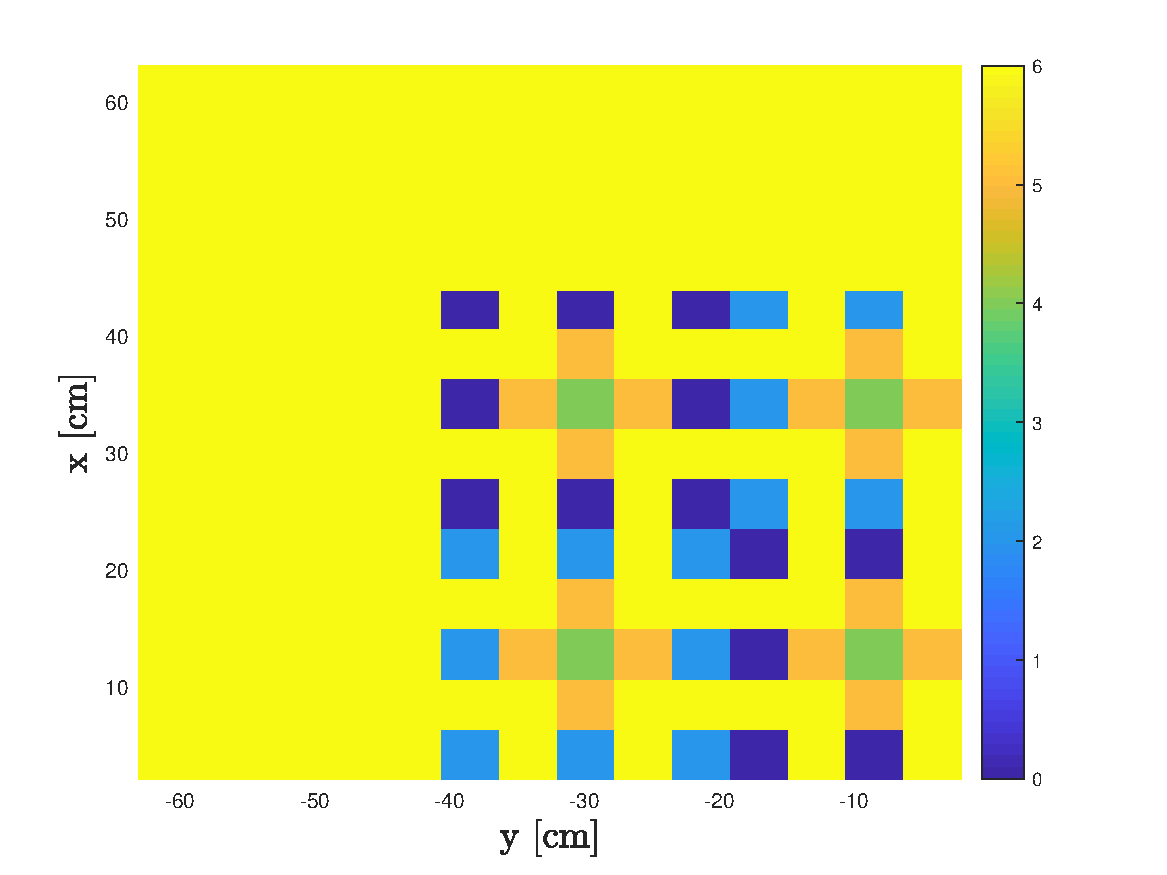
\includegraphics[width=.75\linewidth]{{Figures/HigherDimEigen/MOXAssembly_CoarseMaterial}}
        \caption{Coarse Spatial Homogenization of MOX Fuel Assembly Benchmark Problem}\label{fig:CoarseGeo}
        \caption*{Each material is given a number which corresponds to the color shown in the figure: UO$_{2}$ = 0, 4.3\% MOX Fuel = 1, 7.0\% MOX Fuel = 2, 8.7\% MOX Fuel = 3, Guide Tube = 4, Fission Chamber = 5, Moderator = 6.}
\end{figure}

\clearpage

For the alpha-eigenvalue, the RQFP method required 6776 transport sweeps to converge the eigenvalue/eigenvector residual to a tolerance of $10^{-6}$ as seen in Table~\ref{table:2DMoxCoarseAlpha}. The critical search method required 81445 transport sweeps after requiring seven intermediate $k$-effective calculations. The group scalar fluxes for the seven groups can be seen in Figure~\ref{fig:ScalarFluxCoarse}. The RQFP method was able to converge the alpha-eigenvalue/eigenvector despite the system being highly supercritical. Despite the fact that not all cells contained fissile material and the moderator contained only downscattering, the violation of the primitivity condition did not affect the ability of the method to converge.

For the $k$-effective eigenvalue, the RQFP method required 9064 transport sweeps as compared to 9681 transport sweeps for the power method with fission source norm update (Table~\ref{table:2DMoxCoarseK}). As the problem was substantially supercritical, the performance of the RQFP method was not degraded by the large amounts of scattering in the moderator regions of the problem and converges the solution is fewer iteration than the power method. The $k$-effective eigenvalue group scalar fluxes were substantially different from the alpha-eigenvalue group scalar fluxes as expected since the problem was not close to critical. The absolute difference between the alpha-eigenvalue and $k$-effective eigenvectors for energy group six is seen in Figure~\ref{fig:EigScalarFluxDiff}. The number of transport sweeps necessary to converge the two eigenproblems were noticeable different with the $k$-effective eigenvalue requiring approximately 33\% more sweeps.

\begin{table}[!htbp]
	\caption{Calculated Eigenvalues and Transport Sweep Comparisons for Two-Dimensional MOX Fuel Core with Coarse Spatial Discretization}
	\label{table:2DMOXCoarseRes}
	\begin{subtable}[h]{1.0\textwidth}
	\centering\ra{1.3}
	\begin{tabular}{@{}cccc@{}}\toprule
	& & \multicolumn{2}{c}{Transport Sweeps} \\
	\cmidrule{3-4} Benchmark Problem & Calculated $\alpha$ [$\mu$s$^{-1}$] & RQFP & Critical Search\\
	\midrule
	2D MOX Coarse Discretization & $1.492999 \times 10^{-1}$ & 6776 & 81445 \\
	\bottomrule
	\end{tabular}
	\caption{Alpha-Eigenvalue: Comparison of RQFP and Critical Search Transport Sweeps}
	\label{table:2DMoxCoarseAlpha}
	\end{subtable}%
	\vspace{0.25cm}
	\begin{subtable}[h]{1.0\textwidth}
	\centering\ra{1.3}
	\begin{tabular}{@{}ccccc@{}}\toprule
	& & \multicolumn{2}{c}{Transport Sweeps} \\
	\cmidrule{3-4} Benchmark Problem & Calculated $k_{\text{eff}}$ & RQFP & Power Method \\
	\midrule
	2D MOX Coarse Discretization  & 1.184977 & 9064 & 9681 \\
	\bottomrule
	\multicolumn{4}{l}{$M = 20 \times 20$, $L = 16$, Tolerance = $10^{-6}$} \\
	\end{tabular}
	\caption{$k$-Effective: Comparison of RQFP and Power Method Transport Sweeps}
	\label{table:2DMoxCoarseK}
	\end{subtable}
\end{table}

\clearpage

\begin{figure}[!htbp]
\centering
\begin{subfigure}{.5\textwidth}
  \centering
  \includegraphics[width=.8\linewidth]{{Figures/HigherDimEigen/AlphaScalarFluxRQ_g=0}}
        \caption{Scalar Flux for Energy Group Zero}
  \label{fig:2DAlpha0}
\end{subfigure}%
\begin{subfigure}{.5\textwidth}
  \centering
  \includegraphics[width=.8\linewidth]{{Figures/HigherDimEigen/AlphaScalarFluxRQ_g=1}}
        \caption{Scalar Flux for Energy Group One}
  \label{fig:2DAlpha1}
\end{subfigure}
\begin{subfigure}{.5\textwidth}
  \centering
  \includegraphics[width=.8\linewidth]{{Figures/HigherDimEigen/AlphaScalarFluxRQ_g=2}}
        \caption{Scalar Flux for Energy Group Two}
  \label{fig:2DAlpha2}
\end{subfigure}%
\begin{subfigure}{.5\textwidth}
  \centering
  \includegraphics[width=.8\linewidth]{{Figures/HigherDimEigen/AlphaScalarFluxRQ_g=3}}
        \caption{Scalar Flux for Energy Group Three}
  \label{fig:2DAlpha3}
\end{subfigure}
\begin{subfigure}{.5\textwidth}
  \centering
  \includegraphics[width=.8\linewidth]{{Figures/HigherDimEigen/AlphaScalarFluxRQ_g=4}}
        \caption{Scalar Flux for Energy Group Four}
  \label{fig:2DAlpha4}
\end{subfigure}%
\begin{subfigure}{.5\textwidth}
  \centering
  \includegraphics[width=.8\linewidth]{{Figures/HigherDimEigen/AlphaScalarFluxRQ_g=5}}
        \caption{Scalar Flux for Energy Group Five}
  \label{fig:2DAlpha5}
\end{subfigure}
%\caption{A figure with two subfigures}
%\label{fig:test}
\end{figure}

\begin{figure}[!htbp]\ContinuedFloat
\centering
\begin{subfigure}{\textwidth}
  \centering
  \includegraphics[width=.7\linewidth]{{Figures/HigherDimEigen/AlphaScalarFluxRQ_g=6}}
        \caption{Scalar Flux for Energy Group Six}
  \label{fig:2DAlpha6}
\end{subfigure}
\caption{Alpha-Eigenvalue Group Scalar Flux for 2D MOX Fuel Assembly Benchmark Problem - Coarse Spatial Discretization}
\label{fig:ScalarFluxCoarse}
\end{figure}

\begin{figure}[!htbp]
\centering
\begin{subfigure}{\textwidth}
  \centering
  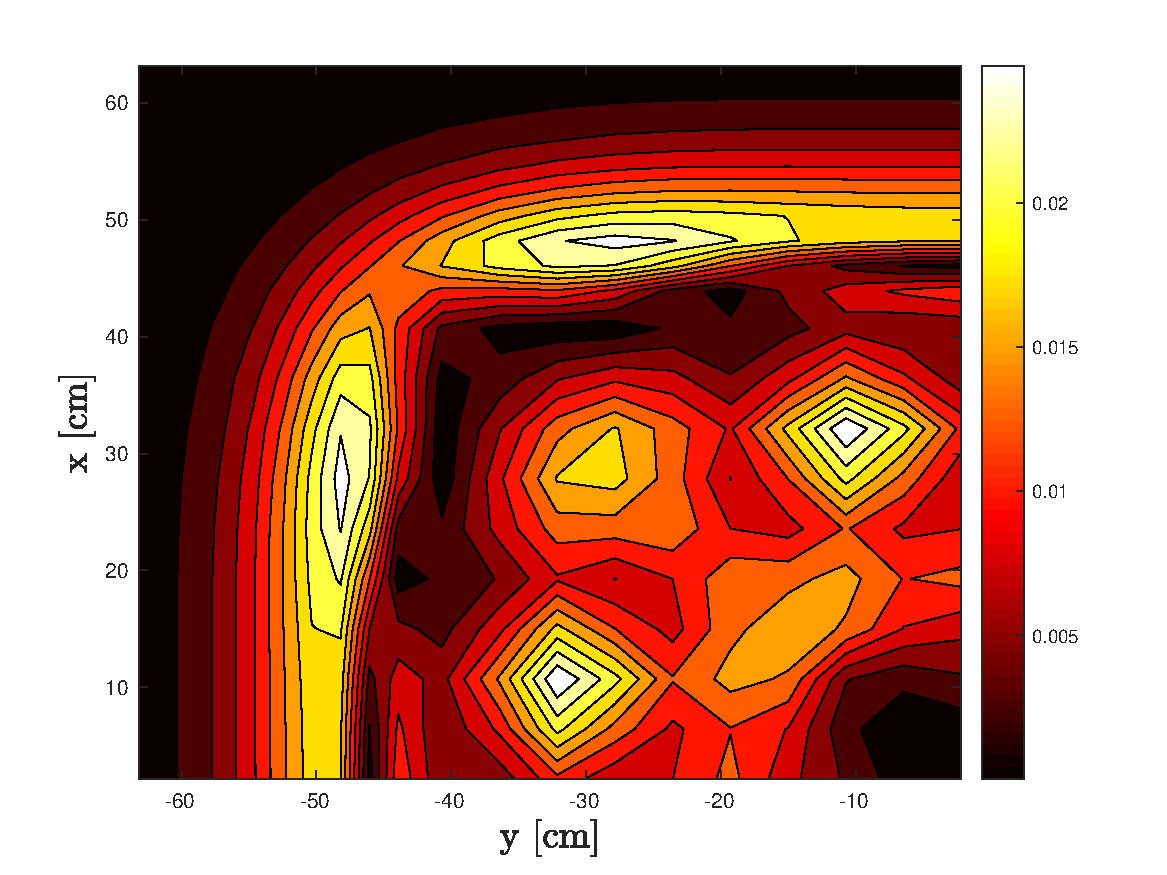
\includegraphics[width=.7\linewidth]{Figures/HigherDimEigen/Alpha_g6_k_g6_AbsDiff}
\end{subfigure}
\caption{Absolute Difference between Alpha-Eigenvalue and $k$-Effective Eigenvalue Group Six Scalar Flux (Coarse Homogenization)}
\label{fig:EigScalarFluxDiff}
\end{figure}

\clearpage
\subsection{Two-Dimensional MOX Fuel Core with Fine Spatial Discretization}

A fine spatial homogenization of the benchmark led to the assembly geometry shown in Figure~\ref{fig:FineGeo}. The fine spatial homogenization allowed for high-fidelity modeling of the assembly, with individual fuel pins, guide tubes, and fission chambers resolved in the model. For the fine spatial discretization diamond differencing was used with 340 spatial cells in both the $x$- and $y$-direction. The problem used S$_{16}$ discrete ordinates angular quadrature. For the fine spatial homogenization, the $k$-effective eigenvalue of the problem was found to be $k = 1.185303$. The alpha-eigenvalue was found to be $\alpha = 1.396240 \times 10^{-1}$ $\mu s^{-1}$. 

\begin{figure}[!htbp]
\centering
  \centering
  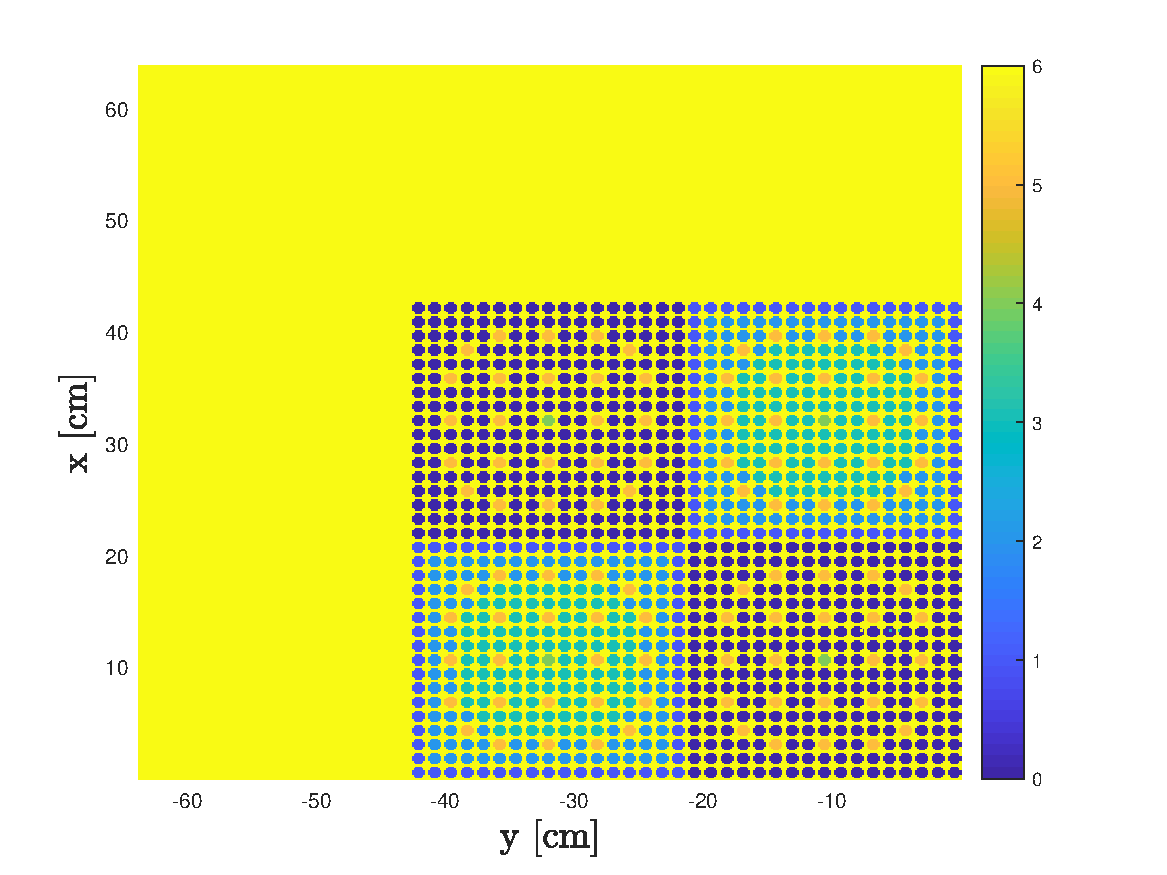
\includegraphics[width=.75\linewidth]{{Figures/HigherDimEigen/MOXAssembly_FineMaterial}}
        \caption{Fine Spatial Homogenization of MOX Fuel Assembly Benchmark Problem}\label{fig:FineGeo}
        \caption*{The color in each cell corresponds to the material in that cell. Each material is given a number which corresponds to the color shown in the figure: UO$_{2}$ = 0, 4.3\% MOX Fuel = 1, 7.0\% MOX Fuel = 2, 8.7\% MOX Fuel = 3, Guide Tube = 4, Fission Chamber = 5, Moderator = 6.}
       % \label{fig:FineGeo}
\end{figure}

\clearpage

Determining the alpha-eigenvalue and eigenvector using the RQFP method required 4096 transport sweeps while the critical search method required 39942 transport sweeps as shown in Table~\ref{table:2DMoxFineAlpha}. The RQFP method reduced the number of transport sweeps necessary to converge the eigenpair to a tolerance of $10^{-6}$ by approximately a factor of ten. The critical search required 12 intermediate $k$-effective eigenvalue calculations. The alpha-eigenvalue group scalar fluxes for all seven groups are shown in Figure~\ref{fig:2DAlphaFine}. Similar to the coarse spatial homogenization problem, the RQFP method is able to resolve the alpha-eigenvalue and eigenvector despite the presence of cells which violate the assumptions made in deriving the method.

For the $k$-effective eigenvalue, the RQFP method required 5579 transport sweeps to converge as compared to 5523 transport sweep for the power method with fission norm update. Unlike the coarse spatial homogenization, the RQFP method underperformed the power method slightly. Despite this, the RQFP method provides another competitive solution method to the eigenvalue problem. As compared to the alpha-eigenvalue RQFP method, the $k$-effective RQFP method required approximately 40\% more transport sweeps to converge the eigenvalue/eigenvector to the same tolerance. This is expected as the fundamental modes are expected to be substantially different as the positive alpha-eigenvalue hardens the neutron energy spectra while the $k$-effective eigenvalue softens the spectrum. The absolute difference between the thermal energy alpha-eigenvalue scalar flux and the thermal energy $k$-effective scalar flux is seen in Figure~\ref{fig:EigScalarFluxDiffFine}.

\begin{table}[!htbp]
	\caption{Calculated Eigenvalues and Transport Sweep Comparisons for Two-Dimensional MOX Fuel Core with Fine Spatial Discretization}
	\label{table:2DMOXFineRes}
	\begin{subtable}[h]{1.0\textwidth}
	\centering\ra{1.3}
	\begin{tabular}{@{}cccc@{}}\toprule
	& & \multicolumn{2}{c}{Transport Sweeps} \\
	\cmidrule{3-4} Benchmark Problem & Calculated $\alpha$ [$\mu$s$^{-1}$] & RQFP & Critical Search\\
	\midrule
	2D MOX Fine Discretization & $1.396240 \times 10^{-1}$ & 4046 & 39942 \\
	\bottomrule
	\end{tabular}
	\caption{Alpha-Eigenvalue: Comparison of RQFP and Critical Search Transport Sweeps}
	\label{table:2DMoxFineAlpha}
	\end{subtable}%
	\vspace{0.25cm}
	\begin{subtable}[h]{1.0\textwidth}
	\centering\ra{1.3}
	\begin{tabular}{@{}ccccc@{}}\toprule
	& & \multicolumn{2}{c}{Transport Sweeps} \\
	\cmidrule{3-4} Benchmark Problem & Calculated $k_{\text{eff}}$ & RQFP & Power Method \\
	\midrule
	2D MOX Fine Discretization  & 1.185303 & 5579 & 5523 \\
	\bottomrule
	\multicolumn{4}{l}{$M = 340 \times 340$, $L = 16$, Tolerance = $10^{-6}$} \\
	\end{tabular}
	\caption{$k$-Effective: Comparison of RQFP and Power Method Transport Sweeps}
	\label{table:2DMoxFineK}
	\end{subtable}
\end{table}

\begin{figure}[!htbp]
\centering
\begin{subfigure}{.5\textwidth}
  \centering
  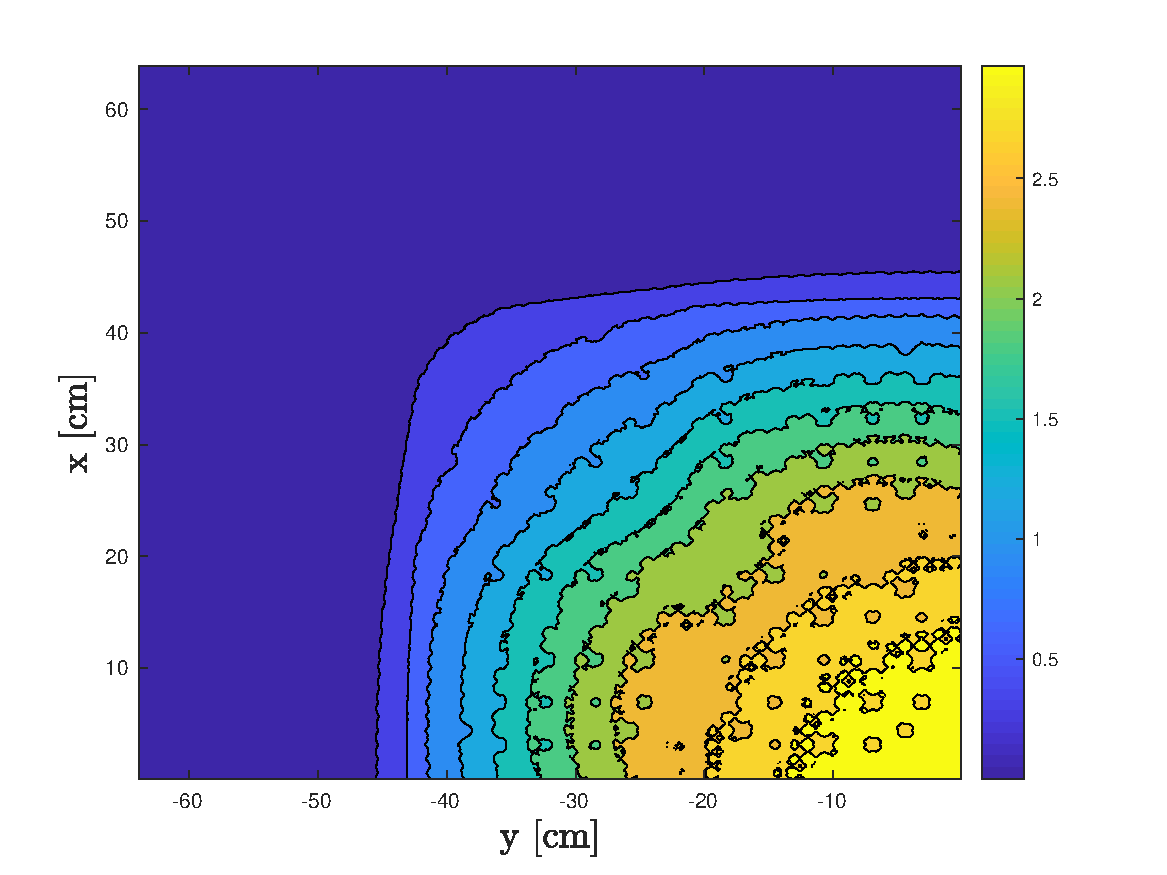
\includegraphics[width=.8\linewidth]{{Figures/HigherDimEigen/AlphaScalarFluxRQ_g_fine=0}}
        \caption{Scalar Flux for Energy Group Zero}
  \label{fig:2DAlpha0Fine}
\end{subfigure}%
\begin{subfigure}{.5\textwidth}
  \centering
  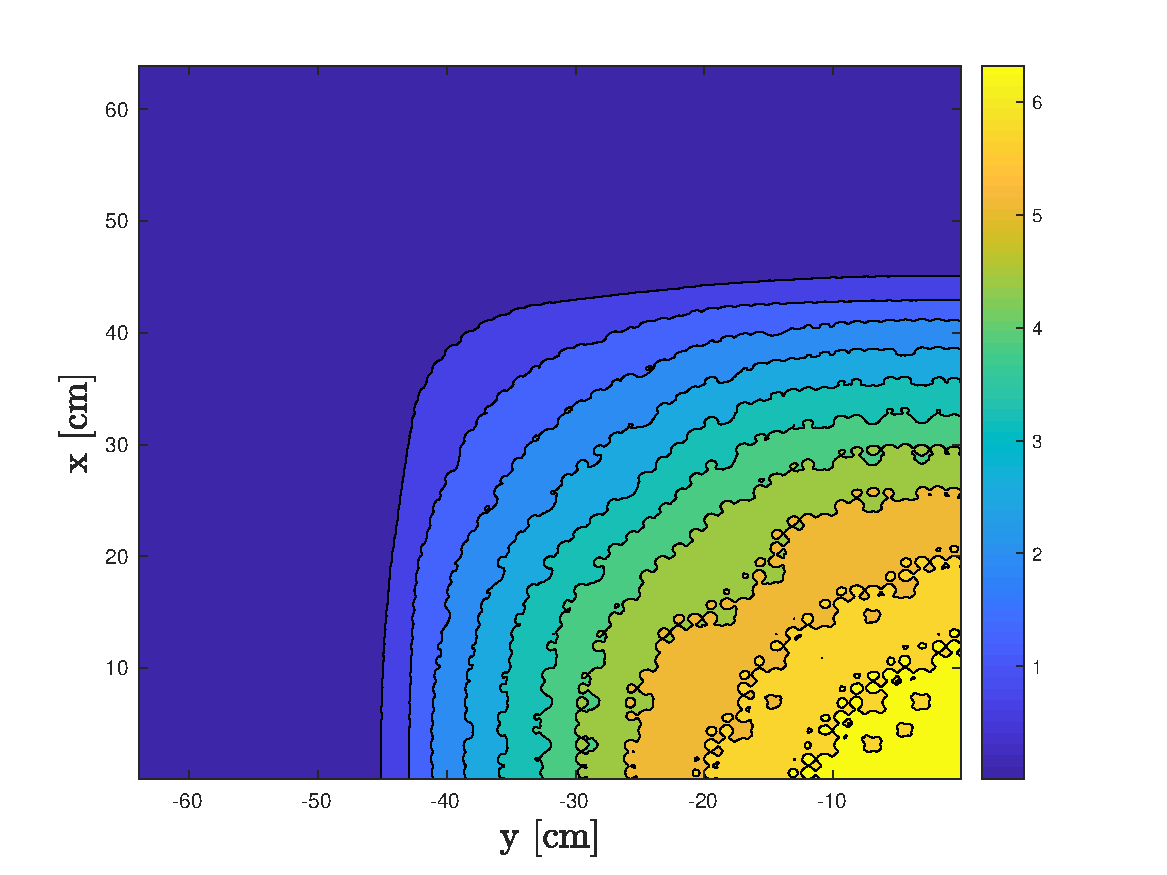
\includegraphics[width=.8\linewidth]{{Figures/HigherDimEigen/AlphaScalarFluxRQ_g_fine=1}}
        \caption{Scalar Flux for Energy Group One}
  \label{fig:2DAlpha1Fine}
\end{subfigure}
\begin{subfigure}{.5\textwidth}
  \centering
  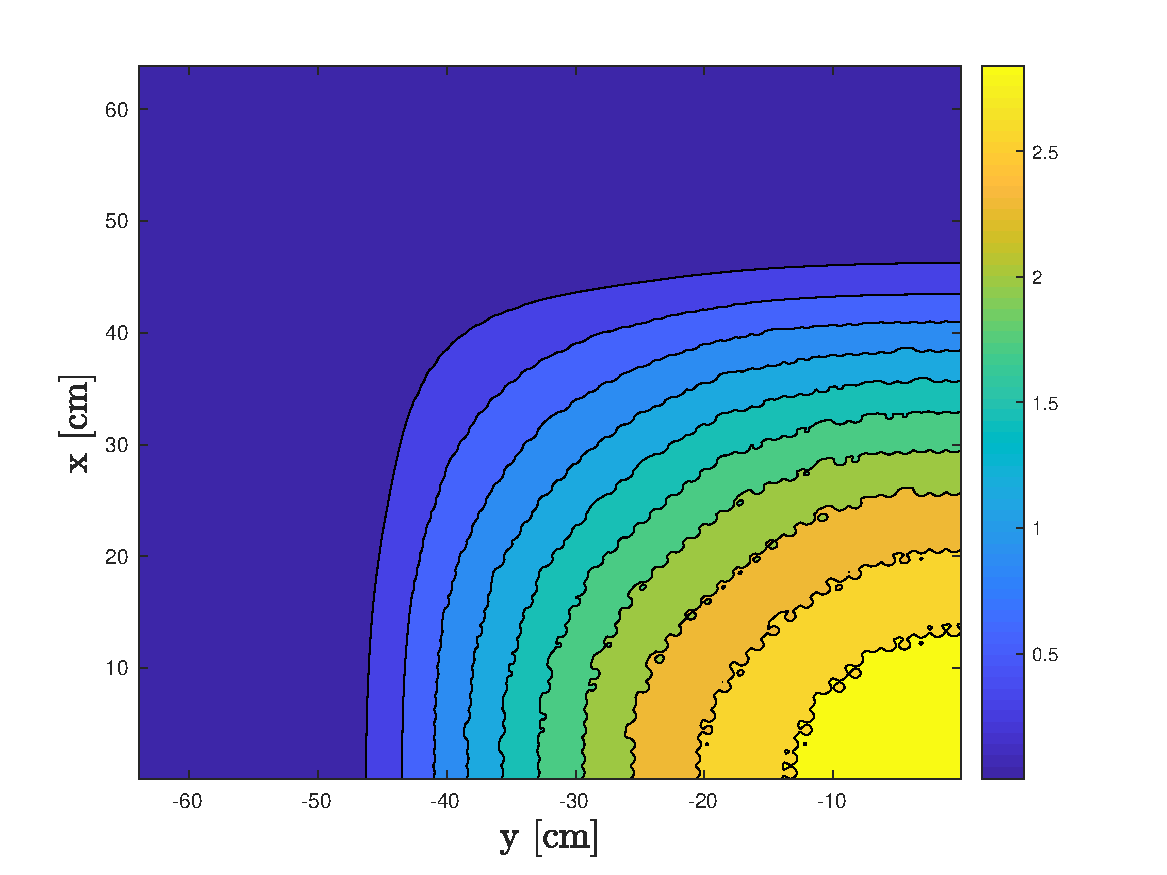
\includegraphics[width=.8\linewidth]{{Figures/HigherDimEigen/AlphaScalarFluxRQ_g_fine=2}}
        \caption{Scalar Flux for Energy Group Two}
  \label{fig:2DAlpha2Fine}
\end{subfigure}%
\begin{subfigure}{.5\textwidth}
  \centering
  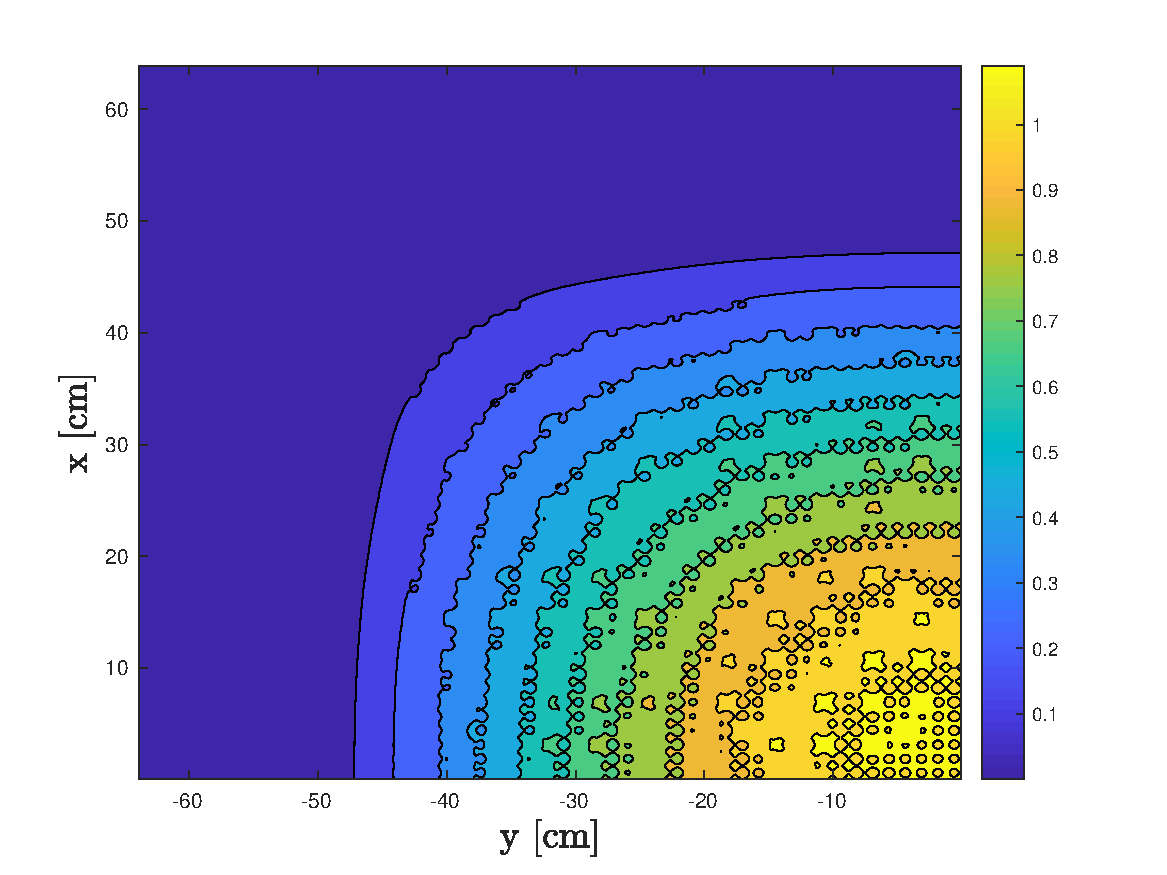
\includegraphics[width=.8\linewidth]{{Figures/HigherDimEigen/AlphaScalarFluxRQ_g_fine=3}}
        \caption{Scalar Flux for Energy Group Three}
  \label{fig:2DAlpha3Fine}
\end{subfigure}
\begin{subfigure}{.5\textwidth}
  \centering
  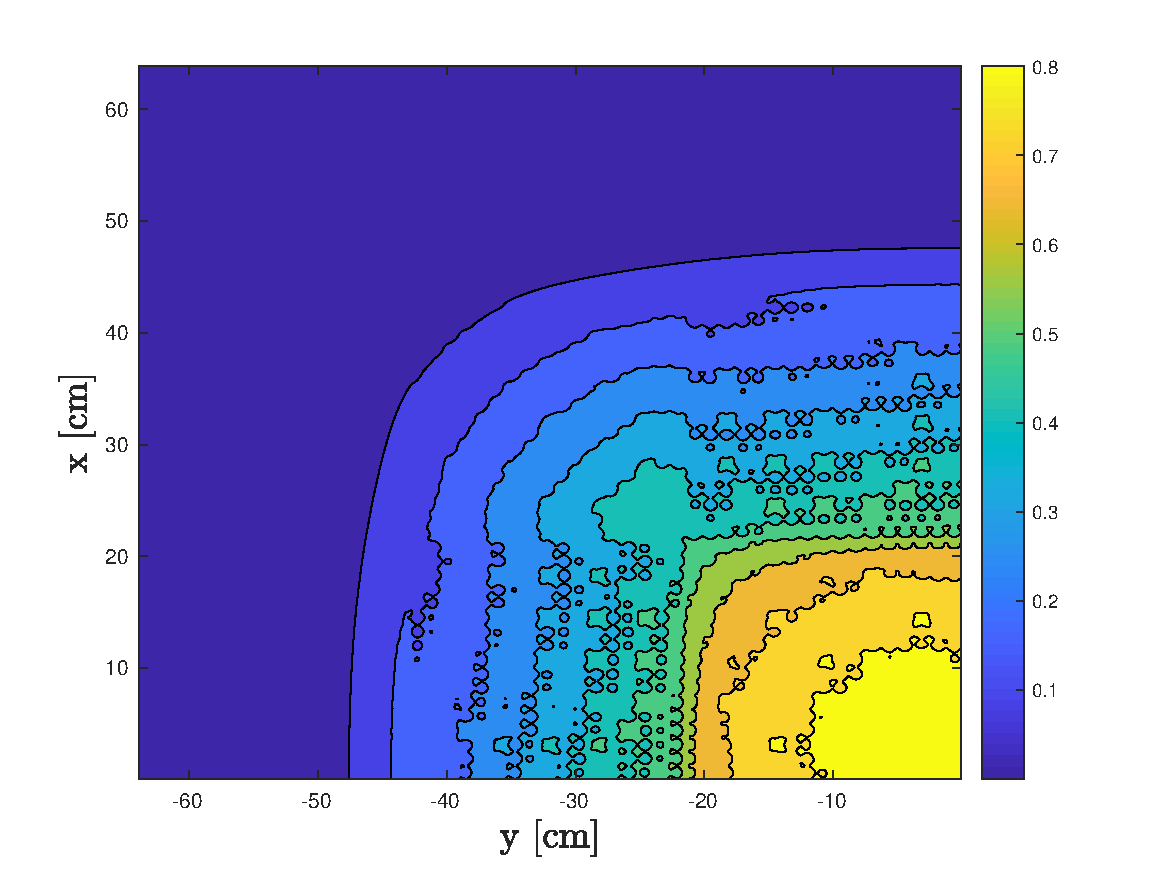
\includegraphics[width=.8\linewidth]{{Figures/HigherDimEigen/AlphaScalarFluxRQ_g_fine=4}}
        \caption{Scalar Flux for Energy Group Four}
  \label{fig:2DAlpha4Fine}
\end{subfigure}%
\begin{subfigure}{.5\textwidth}
  \centering
  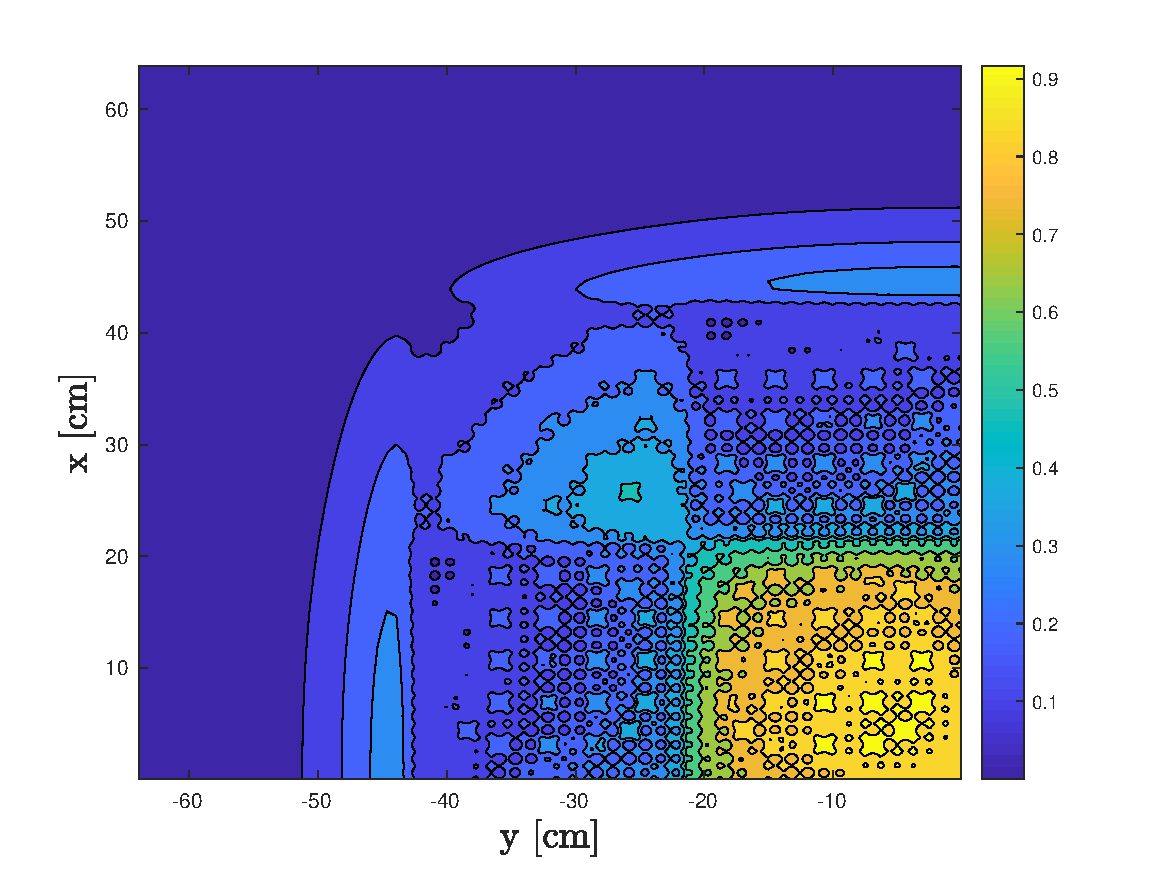
\includegraphics[width=.8\linewidth]{{Figures/HigherDimEigen/AlphaScalarFluxRQ_g_fine=5}}
        \caption{Scalar Flux for Energy Group Five}
  \label{fig:2DAlpha5Fine}
\end{subfigure}
%\caption{A figure with two subfigures}
%\label{fig:test}
\end{figure}

\begin{figure}[!htbp]\ContinuedFloat
\centering
\begin{subfigure}{\textwidth}
  \centering
  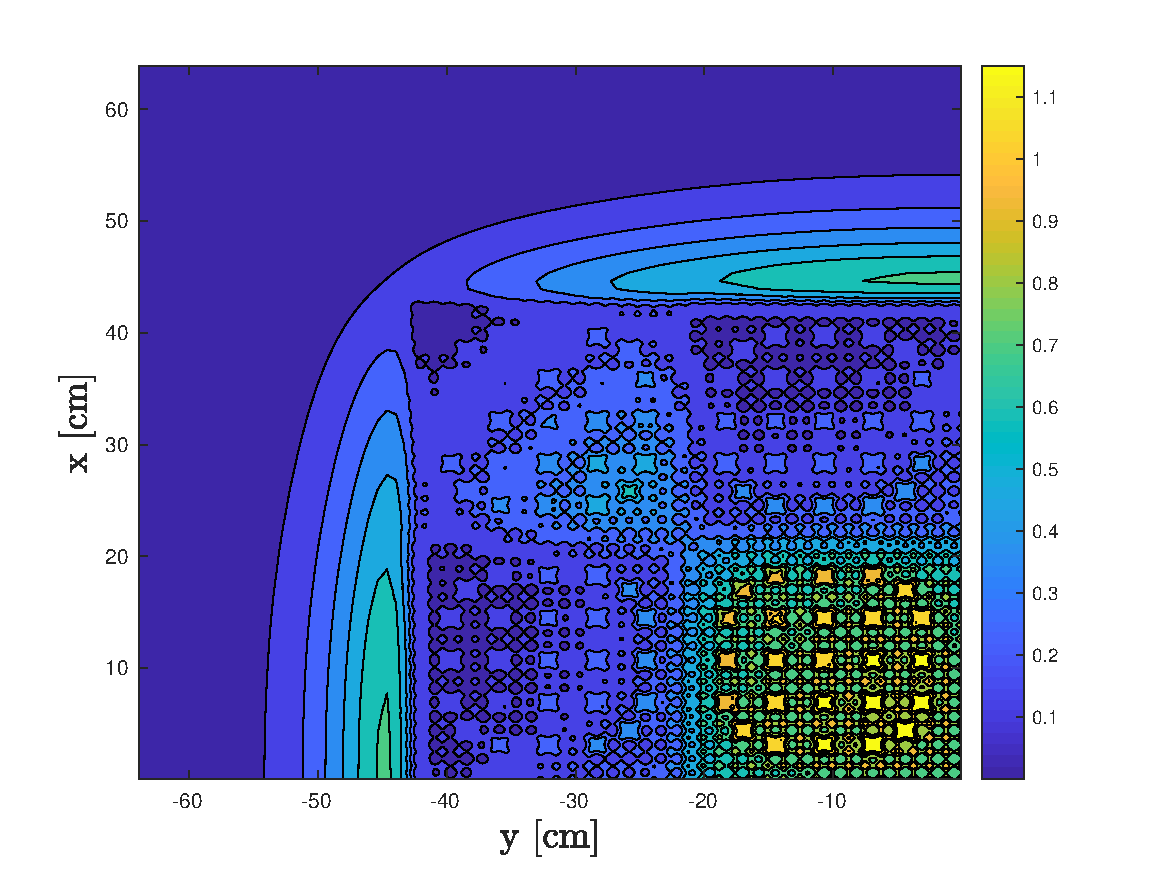
\includegraphics[width=.7\linewidth]{{Figures/HigherDimEigen/AlphaScalarFluxRQ_g_fine=6}}
        \caption{Scalar Flux for Energy Group Six}
  \label{fig:2DAlpha6Fine}
\end{subfigure}
\caption{Alpha-Eigenvalue Group Scalar Flux for 2D MOX Fuel Assembly Benchmark Problem - Fine Spatial Discretization}
\label{fig:2DAlphaFine}
\end{figure}

\begin{figure}[!htbp]
\centering
\begin{subfigure}{\textwidth}
  \centering
  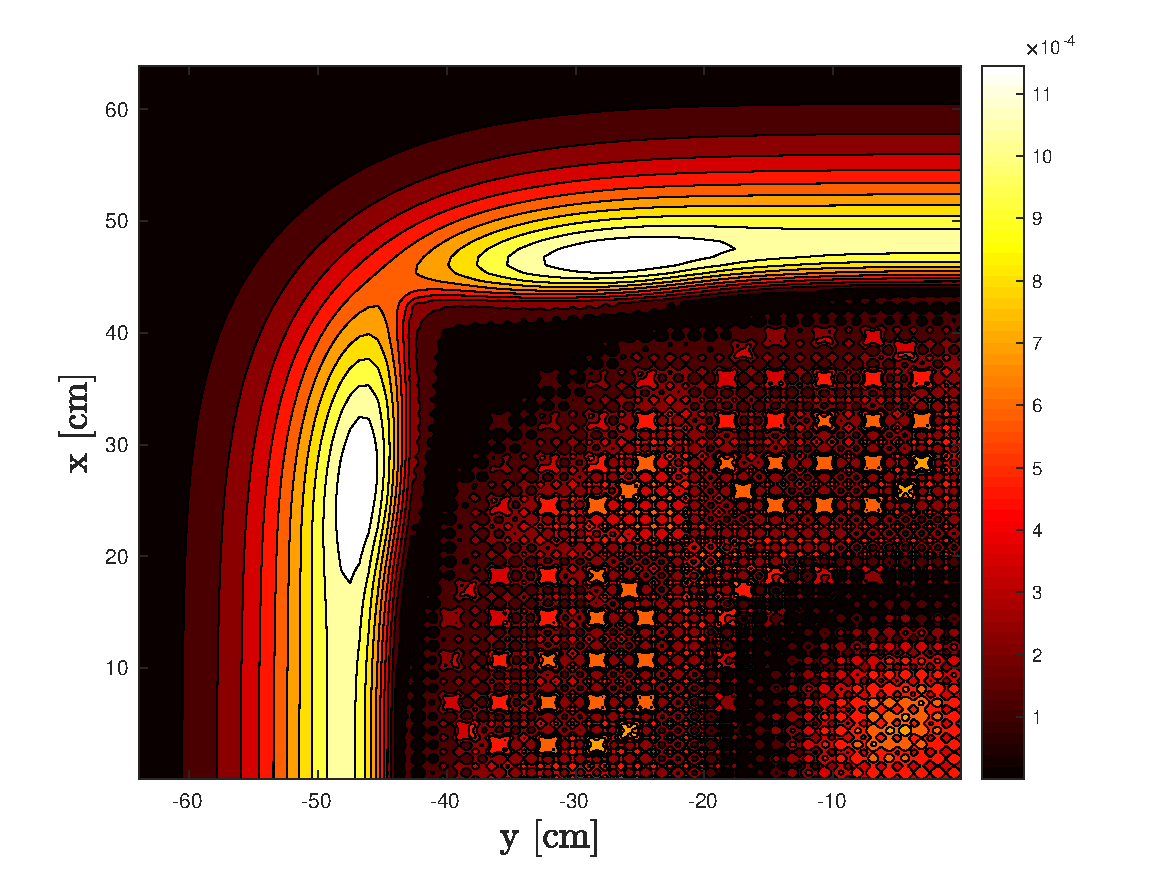
\includegraphics[width=.7\linewidth]{Figures/HigherDimEigen/Alpha_g6_k_g6_FineAbsDiff}
\end{subfigure}
\caption{Absolute Difference between Alpha-Eigenvalue and $k$-Effective Eigenvalue Group Six Scalar Flux (Fine Homogenization)}
\label{fig:EigScalarFluxDiffFine}
\end{figure}

\subsection{Three-Dimensional MOX Fuel Core with Coarse Spatial Discretization}

A coarse spatial homogenization of the three-dimensional quarter core benchmark led to the assembly geometry shown in Figure~\ref{fig:CoarseGeo3D}. Spatial discretization was done using the diamond difference method with the coarse spatial homogenization using twenty cells in the x-, y-, and z-directions each. This benchmark problem used S$_{8}$ discrete ordinates angular quadrature. A reflective boundary condition was placed on the bottom of the assembly and a vacuum boundary condition was placed on the top of the assembly. The $k$-effective eigenvalue of this assembly benchmark model was $k = 1.182340$, slightly more subcritical than the benchmark $k$-effective of $k = 1.186550$. The alpha-eigenvalue of the benchmark was $\alpha = 1.467369 \times 10^{-1}$ $\mu s^{-1}$.

\begin{figure}[!htbp]
\centering
  \centering
  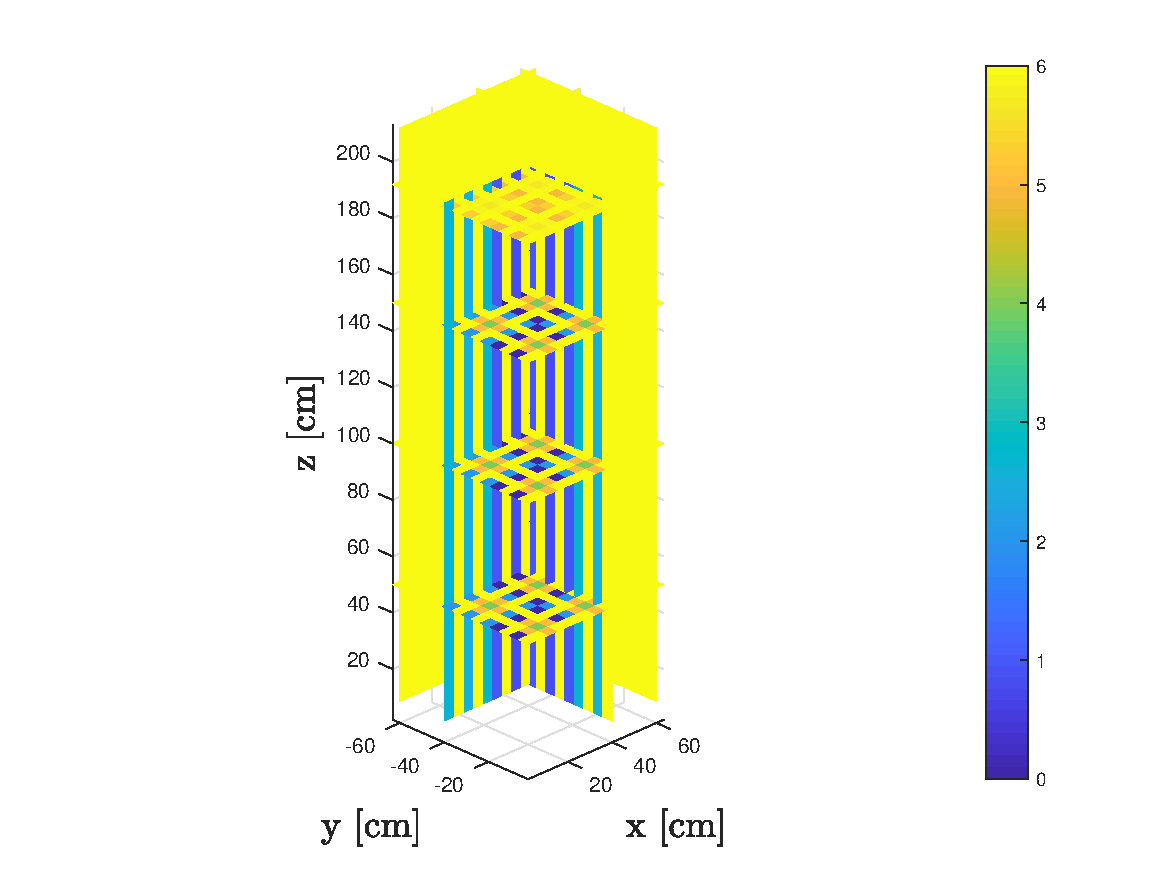
\includegraphics[width=.75\linewidth]{{Figures/HigherDimEigen/MOXAssembly_3d_small}}
        \caption{Coarse Spatial Homogenization of Three-Dimensional MOX Fuel Assembly Benchmark Problem}        \label{fig:CoarseGeo3D}
        \caption*{The color in each cell corresponds to the material in that cell. Each material is given a number which corresponds to the color shown in the figure: UO$_{2}$ = 0, 4.3\% MOX Fuel = 1, 7.0\% MOX Fuel = 2, 8.7\% MOX Fuel = 3, Guide Tube = 4, Fission Chamber = 5, Moderator = 6.}
\end{figure}

\clearpage

To determine the alpha-eigenvalue and eigenvector of the three-dimensional assembly problem to a tolerance of $10^{-6}$, the RQFP method required 38521 transport sweeps as compared to 286566 transport sweeps for the critical search method as shown in Table~\ref{table:3DMOXCoarseAlpha}. The critical search method required 12 $k$-effective eigenvalue calculations in order to converge the alpha-eigenvalue and eigenvector, with some individual $k$-effective calculations requiring a similar number of transport sweeps as the RQFP method. The alpha-eigenvalue group scalar fluxes are seen in Figure~\ref{fig:3DAlphaCoarse}.

The RQFP method required 43309 transport sweeps to converge the $k$-effective eigenvalue and eigenvector (Table~\ref{table:3DMOXCoarseK}). The power method with fission source update required 43666 transport sweeps. Both methods were converged to a tolerance of $10^{-6}$. The RQFP method performed slightly better than the power method for the three-dimensional fuel assembly benchmark problem. Compared to the alpha-eigenvalue problem, the RQFP method required approximately 12\% more transport sweeps to converge the $k$-effective eigenvalue and eigenvector to the same tolerance.

\begin{table}[!htbp]
	\caption{Calculated Eigenvalues and Transport Sweep Comparisons for Three-Dimensional MOX Fuel Core with Coarse Spatial Discretization}
	\label{table:3DMOXCoarseRes}
	\begin{subtable}[h]{1.0\textwidth}
	\centering\ra{1.3}
	\begin{tabular}{@{}cccc@{}}\toprule
	& & \multicolumn{2}{c}{Transport Sweeps} \\
	\cmidrule{3-4} Benchmark Problem & Calculated $\alpha$ [$\mu$s$^{-1}$] & RQFP & Critical Search\\
	\midrule
	3D MOX Coarse Discretization & $1.467369 \times 10^{-1}$ & 38521 & 286566 \\
	\bottomrule
	\end{tabular}
	\caption{Alpha-Eigenvalue: Comparison of RQFP and Critical Search Transport Sweeps}
	\label{table:3DMOXCoarseAlpha}
	\end{subtable}%
	\vspace{0.25cm}
	\begin{subtable}[h]{1.0\textwidth}
	\centering\ra{1.3}
	\begin{tabular}{@{}ccccc@{}}\toprule
	& & \multicolumn{2}{c}{Transport Sweeps} \\
	\cmidrule{3-4} Benchmark Problem & Calculated $k_{\text{eff}}$ & RQFP & Power Method \\
	\midrule
	3D MOX Coarse Discretization & 1.182330 & 43309 & 43666 \\
	\bottomrule
	\multicolumn{4}{l}{$M = 20 \times 20 \times 20$, $L = 8$, Tolerance = $10^{-6}$} \\
	\end{tabular}
	\caption{$k$-Effective: Comparison of RQFP and Power Method Transport Sweeps}
	\label{table:3DMOXCoarseK}
	\end{subtable}
\end{table}

\begin{figure}[!htbp]
\centering
\begin{subfigure}{.5\textwidth}
  \centering
  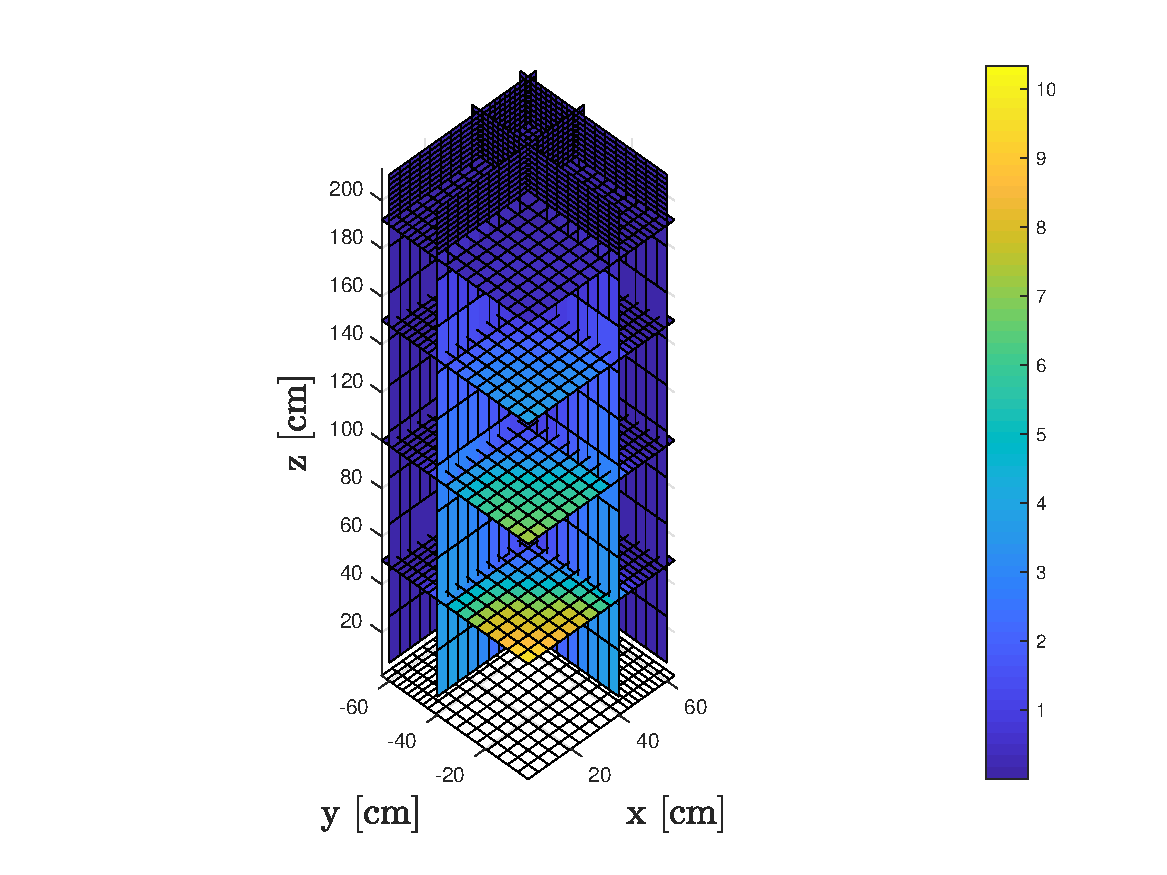
\includegraphics[width=1.\linewidth]{{Figures/HigherDimEigen/AlphaScalarFluxRQ3D_g_coarse=0}}
        \caption{Scalar Flux for Energy Group Zero}
  \label{fig:3DAlpha0Coarse}
\end{subfigure}%
\begin{subfigure}{.5\textwidth}
  \centering
  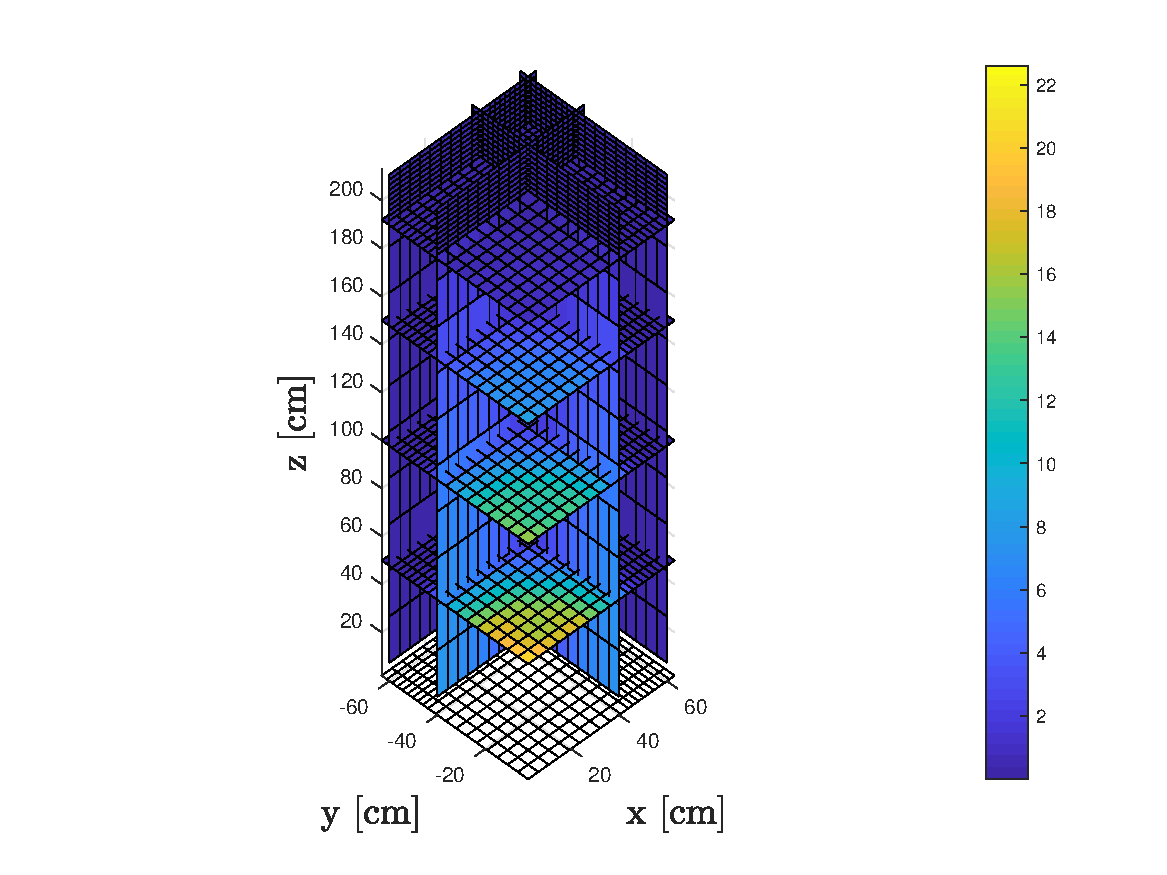
\includegraphics[width=1.\linewidth]{{Figures/HigherDimEigen/AlphaScalarFluxRQ3D_g_coarse=1}}
        \caption{Scalar Flux for Energy Group One}
  \label{fig:3DAlpha1Coarse}
\end{subfigure}
\begin{subfigure}{.5\textwidth}
  \centering
  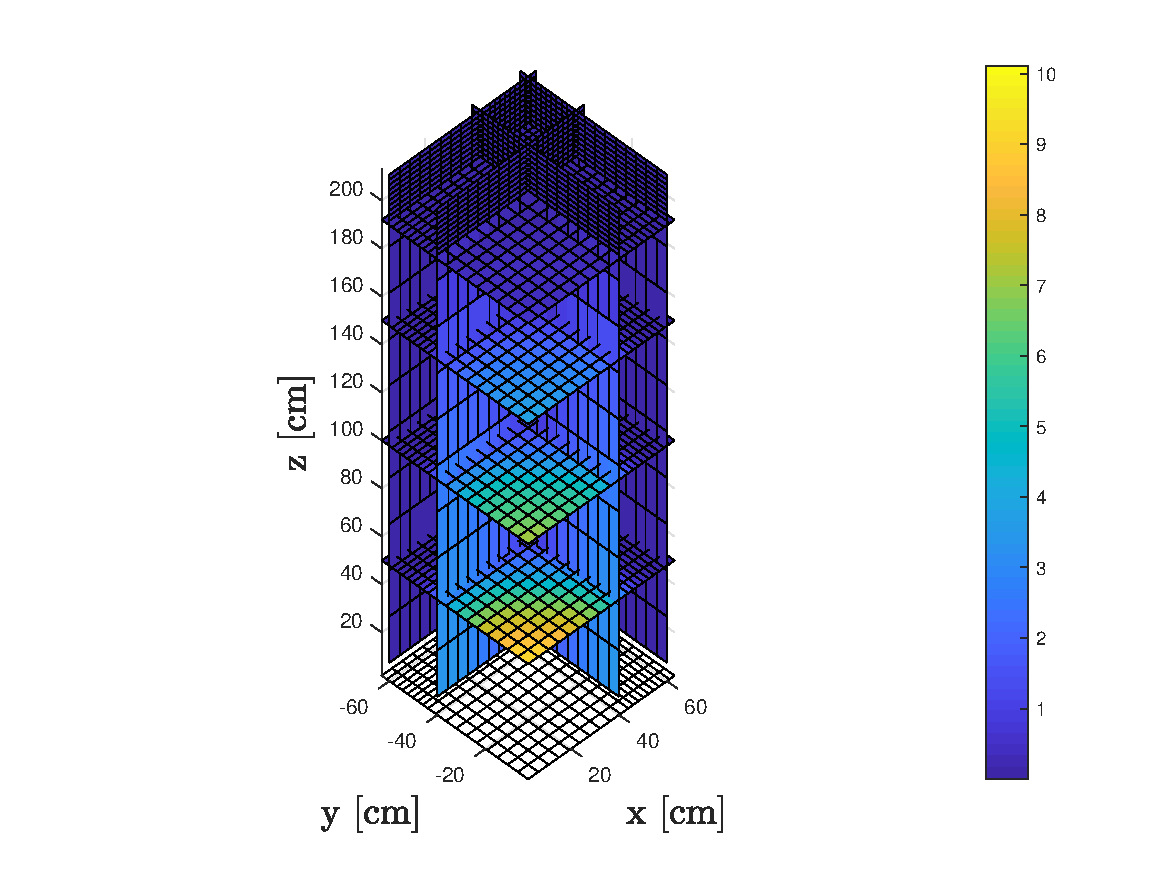
\includegraphics[width=1.\linewidth]{{Figures/HigherDimEigen/AlphaScalarFluxRQ3D_g_coarse=2}}
        \caption{Scalar Flux for Energy Group Two}
  \label{fig:3DAlpha2Coarse}
\end{subfigure}%
\begin{subfigure}{.5\textwidth}
  \centering
  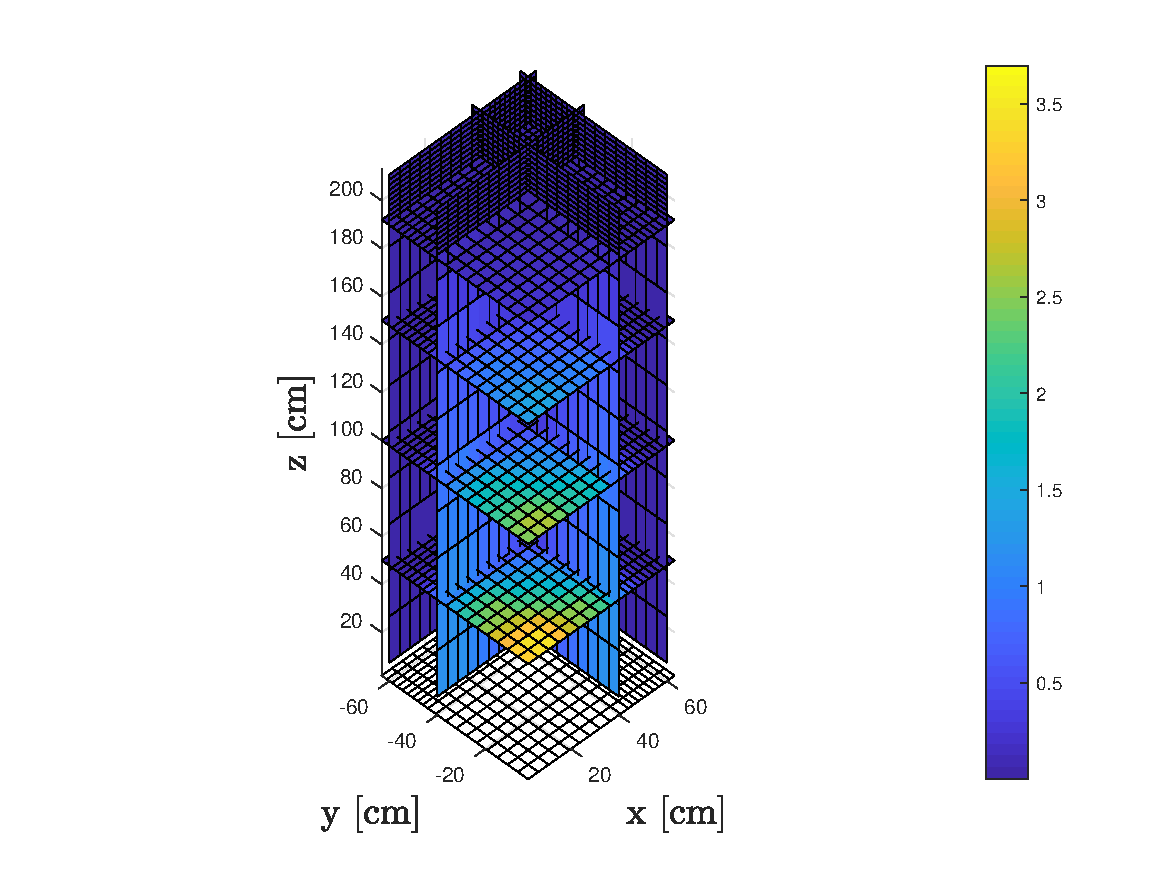
\includegraphics[width=1.\linewidth]{{Figures/HigherDimEigen/AlphaScalarFluxRQ3D_g_coarse=3}}
        \caption{Scalar Flux for Energy Group Three}
  \label{fig:3DAlpha3Coarse}
\end{subfigure}
\begin{subfigure}{.5\textwidth}
  \centering
  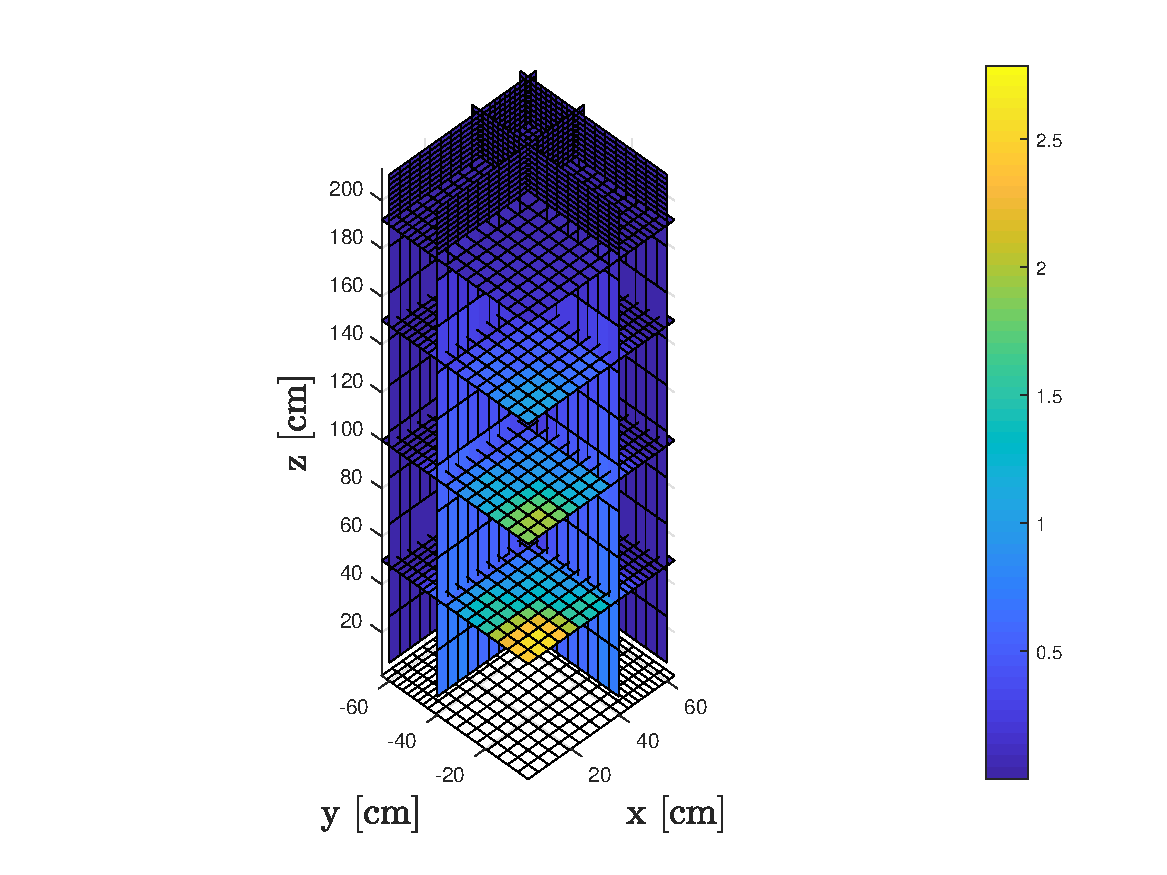
\includegraphics[width=1.\linewidth]{{Figures/HigherDimEigen/AlphaScalarFluxRQ3D_g_coarse=4}}
        \caption{Scalar Flux for Energy Group Four}
  \label{fig:3DAlpha4Coarse}
\end{subfigure}%
\begin{subfigure}{.5\textwidth}
  \centering
  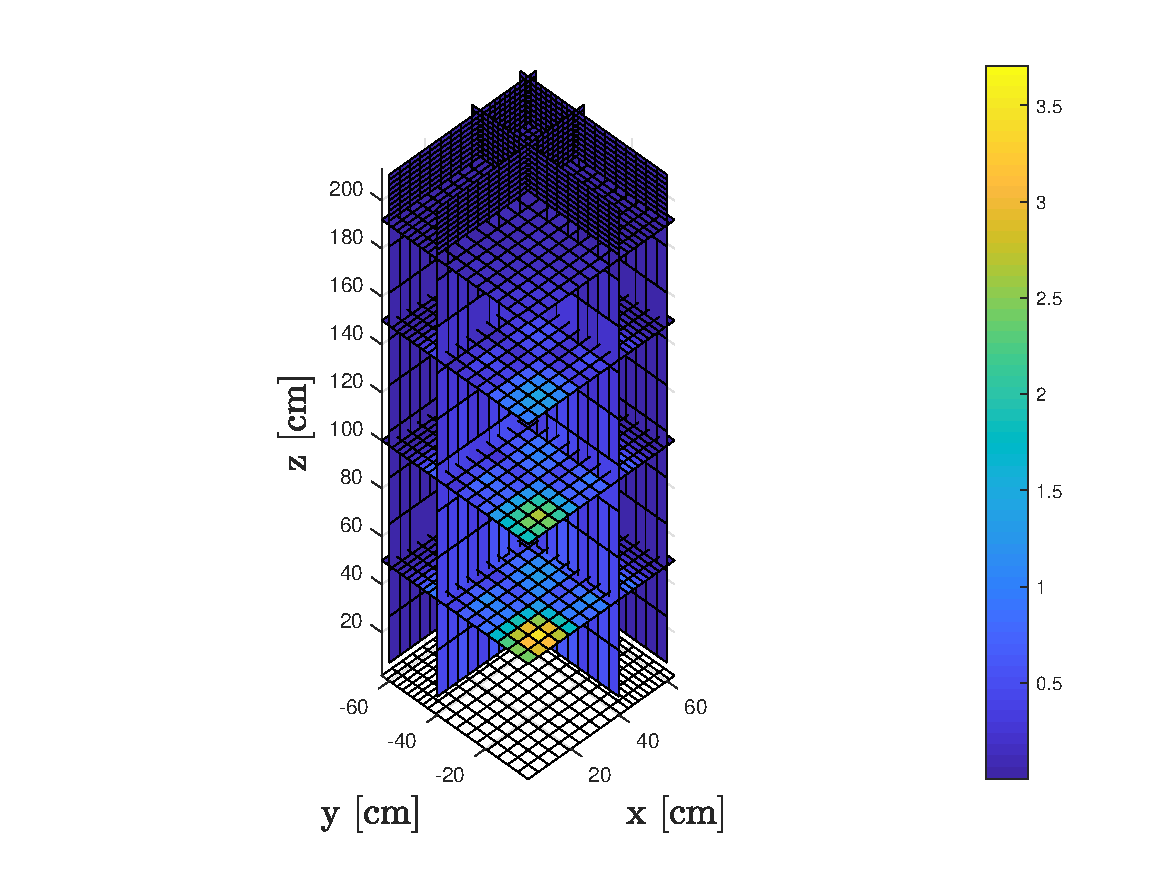
\includegraphics[width=1.\linewidth]{{Figures/HigherDimEigen/AlphaScalarFluxRQ3D_g_coarse=5}}
        \caption{Scalar Flux for Energy Group Five}
  \label{fig:3DAlpha5Coarse}
\end{subfigure}
%\caption{A figure with two subfigures}
%\label{fig:test}
\end{figure}

\begin{figure}[!htbp]\ContinuedFloat
\centering
\begin{subfigure}{\textwidth}
  \centering
  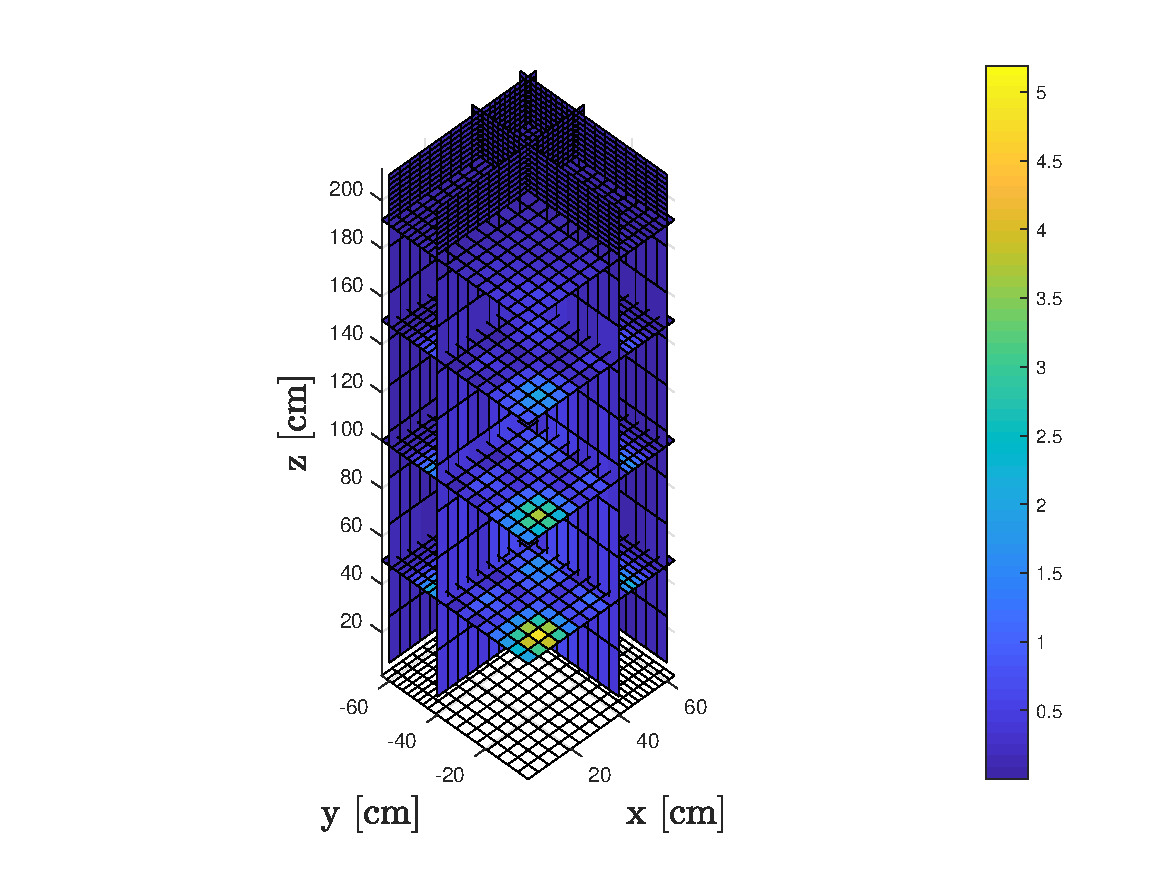
\includegraphics[width=.9\linewidth]{{Figures/HigherDimEigen/AlphaScalarFluxRQ3D_g_coarse=6}}
        \caption{Scalar Flux for Energy Group Six}
  \label{fig:3DAlpha6Coarse}
\end{subfigure}
\caption{Alpha-Eigenvalue Group Scalar Flux for 3D MOX Fuel Assembly Benchmark Problem - Coarse Spatial Discretization}
\label{fig:3DAlphaCoarse}
\end{figure}

%\subsection{Three-Dimensional MOX Fuel Core with Fine Spatial Discretization}

\clearpage

\section{Conclusion}

The Rayleigh Quotient Fixed Point method was applied to alpha- and $k$-effective eigenvalue problems for higher dimensional benchmark problems. Homogeneous critical cylinder problems were examined and the performance of the RQFP method compared to traditional eigensolvers. For alpha-eigenvalue problems, the RQFP method required approximately ten times fewer transport sweeps for critical cylinder problems and was able to converge problems that the critical search method failed to converge. It was found that the rate of convergence of the RQFP method was influenced by the size of the critical system and the amount of scattering present. For $k$-effective eigenvalue problems, the RQFP method required a similar number of transport sweeps as the traditional power method with fission source update. Both the alpha-eigenvalue and $k$-effective eigenvalue RQFP methods required a similar number of iterations for each benchmark as expected due to the similarity of the eigenvectors for both eigenvalue problems.

Three quarter core benchmarks consisting of MOX fuel assemblies were analyzed and the performance of the RQFP method compared to traditional eigensolvers. The criticality eigenvalues of two two-dimensional benchmark problems with coarse and fine spatial homogenization were determined and it was found that the alpha-eigenvalue RQFP method required approximately ten times fewer transport sweeps that the critical search method. The RQFP method for $k$-effective eigenvalues reduced the number of transport sweeps required for convergence by approximately 10\%. For a coarse spatial homogenization three-dimensional benchmark problem, the RQFP method for the alpha-eigenvalue required one-tenth of the transport sweeps required by the critical search method. For the $k$-effective eigenvalue, the RQFP method required fewer iterations than the power method. The RQFP methods were able to determine the fundamental angular flux eigenvector of highly heterogeneous systems. In particular, these systems do not meet all the primitivity requirement made in the derivation of the methods. However, the RQFP method still converges to the eigenvalue and eigenvector of interest and provides substantial reductions in the number of transport sweeps required to converge realistic reactor benchmark problems.